\documentclass[notes]{beamer}
\usetheme{CambridgeUS}
\usepackage[utf8]{inputenc}

\usepackage{pgfpages}
\setbeamertemplate{note page}[default]
\setbeameroption{show notes on second screen=right}
\bibliographystyle{siam}
\usepackage{biblatex}

\title[Synthesis of Circulene]{ Organic Chemistry Final: \\ \large Complete Mechanism for the Synthesis of [7]Circulene}
\author{Cade Reinberger}
\institute[CHCA]{Cincinnati Hills Christian Academy}
\date{\today}

\usepackage{chemfig}
\usepackage{tikz}
\usepackage{mathtools}
\usepackage{relsize}
\usepackage{graphicx}

\date{\today}

\begin{document}

\maketitle

\begin{frame}{[7]Circulene}

\begin{center}
\chemfig{(-[:-90.0,0.759297]-[:-38.571429,0.759297]=^[:25.714286,0.867767]-[:90.0,0.759297]=^[:141.428571,0.759297])-[:25.714286,0.867767](-[:-38.571429,0.759297]-[:12.857143,0.759297]=^[:77.142857,0.867767]-[:141.428571,0.759297]=^[:-167.142857,0.759297])-[:77.142857,0.867767](-[:12.857143,0.759297]-[:64.285714,0.759297]=^[:128.571429,0.867767]-[:-167.142857,0.759297]=^[:-115.714286,0.759297])-[:128.571429,0.867767](-[:64.285714,0.759297]-[:115.714286,0.759297]=^[:180.0,0.867767]-[:-115.714286,0.759297]=^[:-64.285714,0.759297])-[:180.0,0.867767](-[:115.714286,0.759297]-[:167.142857,0.759297]=^[:-128.571429,0.867767]-[:-64.285714,0.759297]=^[:-12.857143,0.759297])-[:-128.571429,0.867767](-[:167.142857,0.759297]-[:-141.428571,0.759297]=^[:-77.142857,0.867767]-[:-12.857143,0.759297]=^[:38.571429,0.759297])-[:-77.142857,0.867767](-[:-141.428571,0.759297]-[:-90.0,0.759297]=^[:-25.714286,0.867767]-[:38.571429,0.759297]=^[:90.0,0.759297])-[:-25.714286,0.867767]}

\note{
\begin{itemize}
    \item Polyaromatic Hydrocarbons ($\approx$ graphene derivatives) are of interest to materials scientists for their electrical properties. Applications like Organic Field-Electron Transistors, and organic photo-voltaic cells. These are of increasing value. \cite{Newswire}
    \item Base-level research in these contorted and geodesic polyarenes are therefore important, and that's a key purpose of molecules like circulen--in the understading of syntheses and reactions of these types of compounds.
\end{itemize}}

\end{center}
\end{frame}

\begin{frame}{Structure}
\begin{center}
    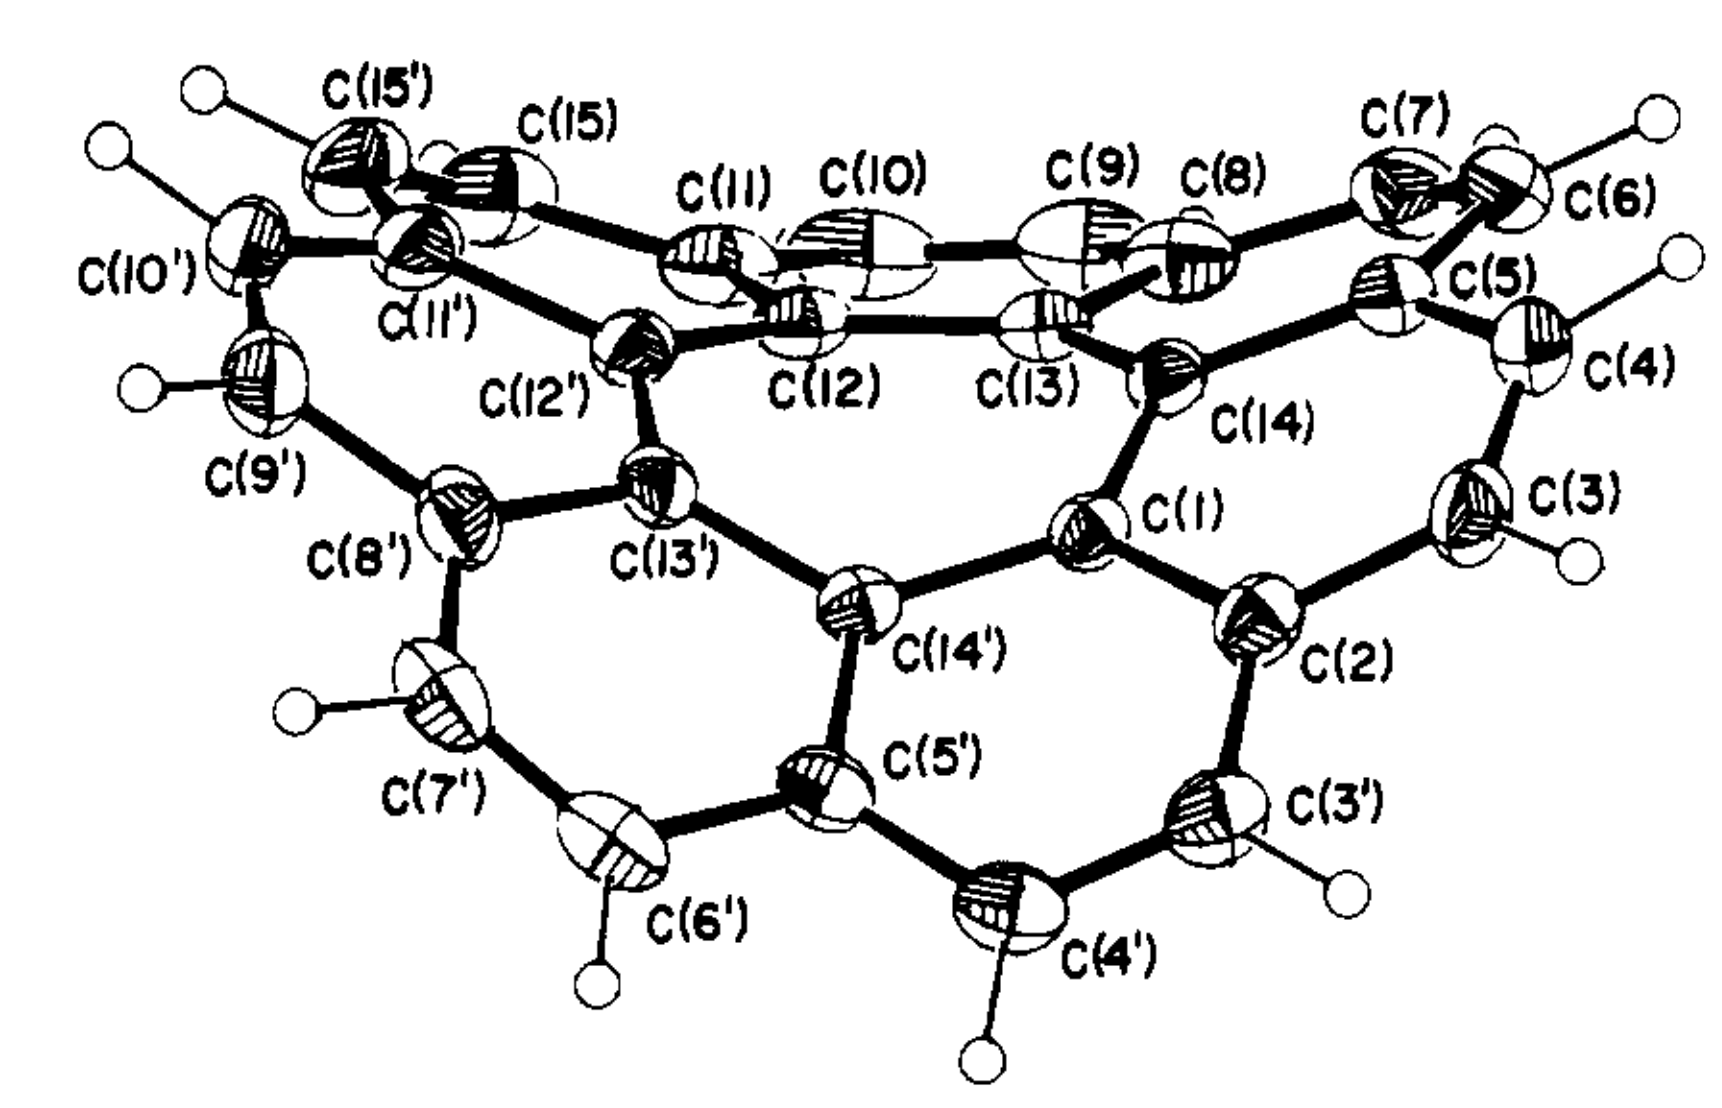
\includegraphics[scale=.5]{seven_circ.PNG}
\end{center}
    
\note{
\begin{itemize}
    \item X-Ray Crystalography shows, shockingly, that the symmetry group is isomorphic to $\mathbb{Z}_2$!
    \item Why would there be contortion? It seems, intuitively that the strain effects, especially for just a 7-membered ring, wouldn't have the same order of magnitude as the effects of stability added when perfectly planar. The answer, digging in to the computer calculation, is twofold. Partly, the resonance stabilization decreases less than you might expect. Partly that's the nature of MO's and linear combination of basis states, but also there's some intuition--think of our dibenzalacetone lab. But, also the ring strain effects add up. There are like 14 involved bonds, so you pick up an order of magnitude in calculation of the strain energy. \cite{Karadakov}
\end{itemize}}
\end{frame}

\begin{frame}{Starting Compound: \textit{5,5'--dimethyl--2,2'--dinitrobiphenyl}}

\begin{figure}
    \centering
    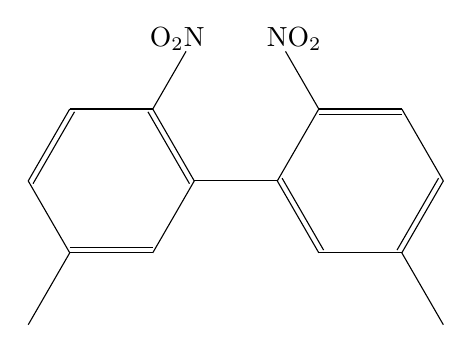
\begin{tikzpicture}[scale=1]
    \schemestart
    \chemfig{=^[:120.0,1.0](-[:60.0,1.0,,2]O_2N)-[:180.0,1.0]=^[:-120.0,1.0]-[:-60.0,1.0](-[:-120.0,1.0])=^[:-0.0,1.0]-[:60.0,1.0]-[:0.0,1.0]=^[:-60.0,1.0]-[:-0.0,1.0](-[:-60.0,1.0])=^[:60.0,1.0]-[:120.0,1.0]=^[:180.0,1.0](-[:120.0,1.0,,1]NO_2)-[:-120.0,1.0]}
    \schemestop
    \end{tikzpicture}
\end{figure}

\note{
\begin{itemize}
    \item Toluene is found in nature, and a byprodct of several key industrial processes, gasoline cracking and the production of steel from coke. Biphenyls are prepared by certain coupling reactions, thereof, so di-methyl-biphenyls are quite natural to work with \cite{Ullman}
    \item Nitration of aromatic compounds has a resonance, and this makes it one of the most common and well-studied among electrophilic aromatic substitutions, which mikes the Nitro compound also a good starting point. \cite{Smith} 
    \item Since the steps of EAS and coupling reactions yield differently directed compounds, it's also far cheaper to buy this as a starting point from a company that will sell other isomers than to synthesize. 
\end{itemize}}

\end{frame}


\begin{frame}{Reduction of Aromatic Nitro Groups}
\begin{center}
    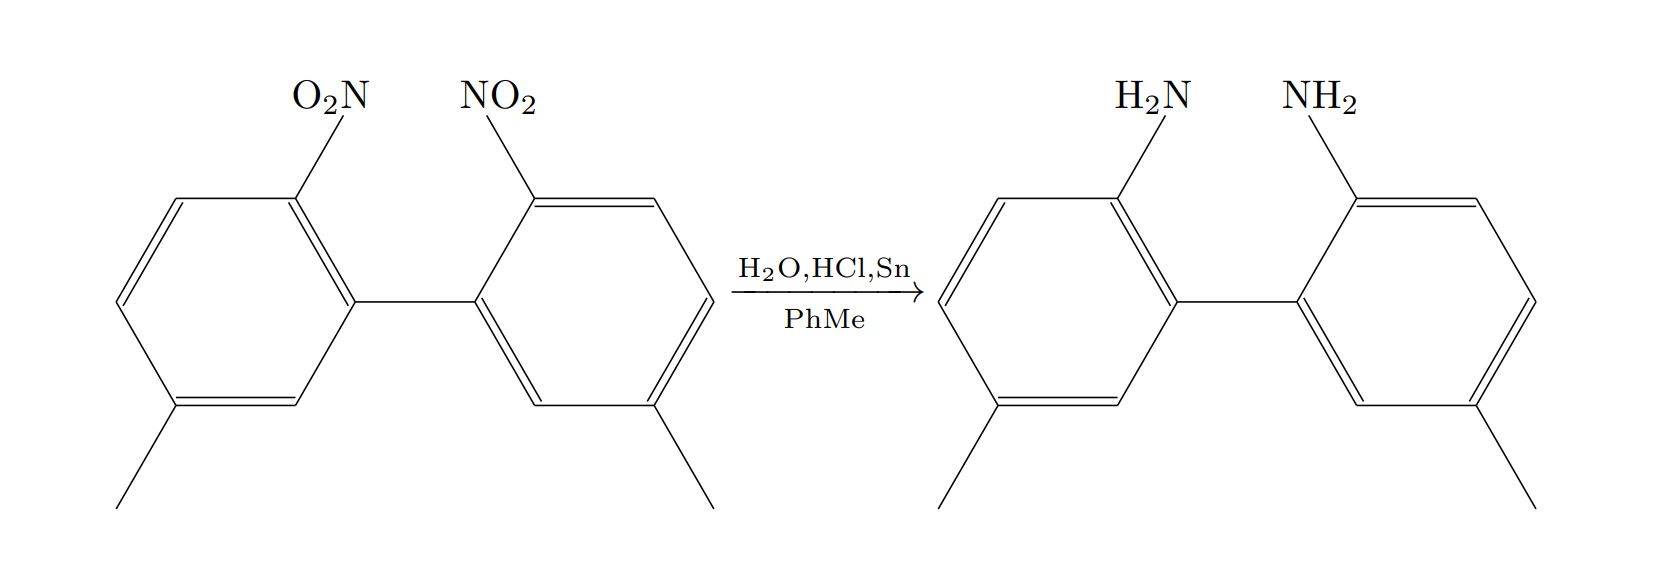
\includegraphics[scale=.25]{aromatic_nitro_reduction_overall.JPG}
\end{center}

\note{
\begin{itemize}
    \item Tin Catalysis with SET--industrially actually want excess of 6 equivalents of Sn. Why? Roughly, Tin has first Ionization energy 708.6 kJ/mol and second ionization energy 1411.8 kJ/mol, so it's usually cheaper to just improve the efficiency and lower the activation energy just by shelling out for the extra equivalents of Tin. 
    \item Single Electron transfer is a special case of a radical mechanism. In the same way that an Sn2 is a special case of a non radical reaction. You can think of it roughly as a radical nucleophilic attack. 
\end{itemize}}

\end{frame}

\begin{frame}{Reduction of Aromatic Nitro Groups: Mechanism \#1}

\begin{center}
    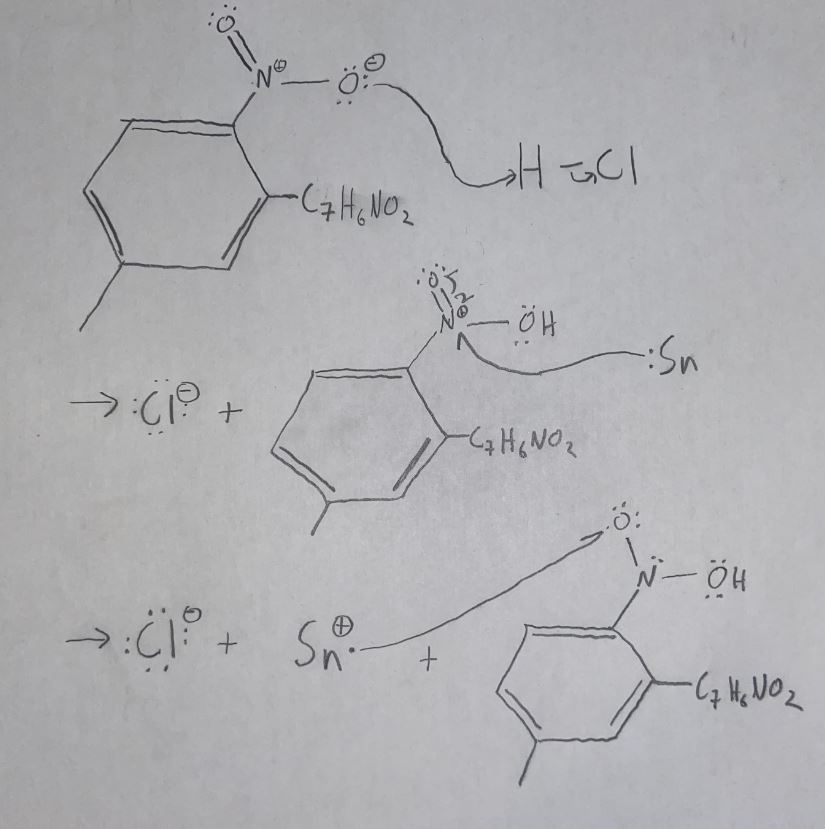
\includegraphics[scale=.3]{aromatic_nitro_reduction_one.JPG}
\end{center}

\note{
\begin{itemize}
    \item attack of the Sn fundamentally nucleophilic though radical. 
    \item second attack could could come from first radical of second Sn if 6 equivalents per nitro. This distinction illustrates SET vs simple nucleophilic attack. 
    \item Though not neccessary, for this first reaction only, since it's so complicated and the equivalents thing is illustrative of the mechanism, we will keep track of all compounds once used. 
\end{itemize}}
\end{frame}

\begin{frame}{Reduction of Aromatic Nitro Groups: Mechanism \#2}
    \begin{center}
        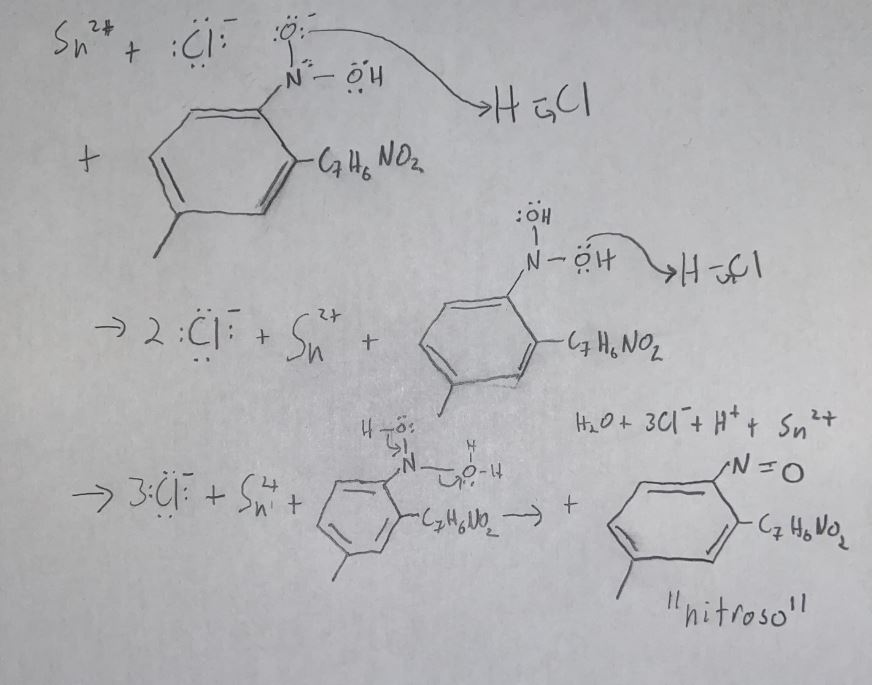
\includegraphics[scale=.35]{aromatic_nitro_reduction_two.JPG}
    \end{center}
    
    \note{
    \begin{itemize}
        \item Nitroso intermediate observed
    \end{itemize}}
\end{frame}

\begin{frame}{Reduction of Aromatic Nitro Groups: Mechanism \#3}
    \begin{center}
        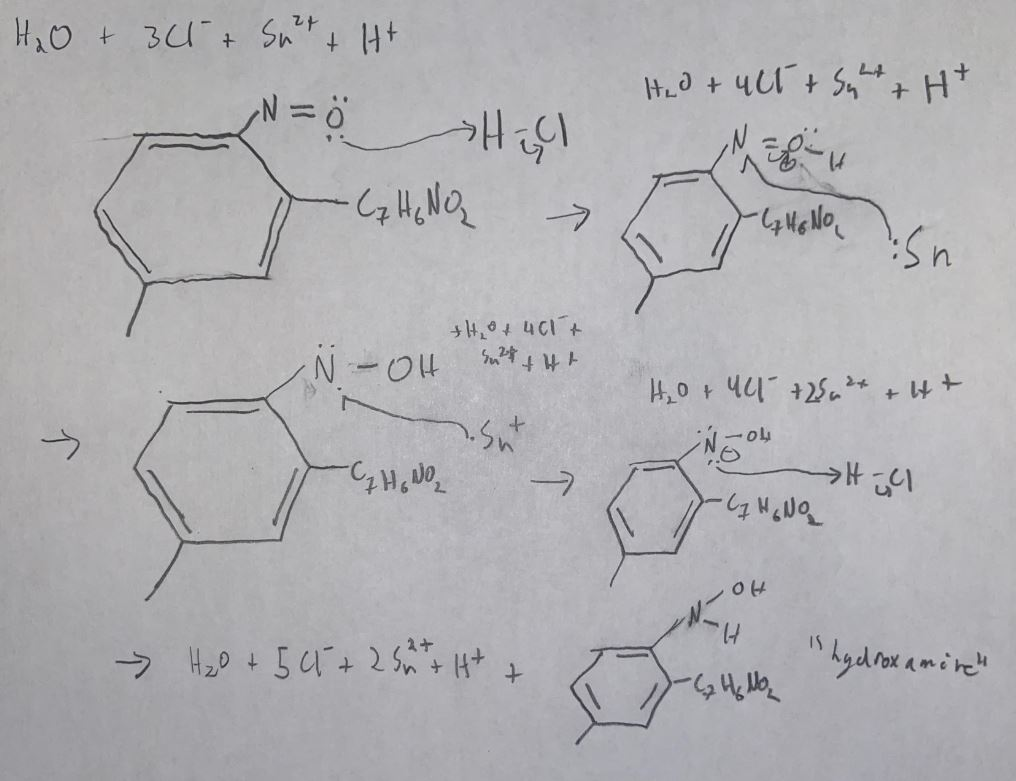
\includegraphics[scale=.35]{aromatic_nitro_reduction_three.JPG}
    \end{center}
    
    \note{
    \begin{itemize}
        \item Donating properties of Nitrogen make Oxygen nucleophilic
        \item Hydroxanamine intermediate observed
    \end{itemize}}
\end{frame}

\begin{frame}{Reduction of Aromatic Nitro Groups: Mechanism \#4}
    \begin{center}
        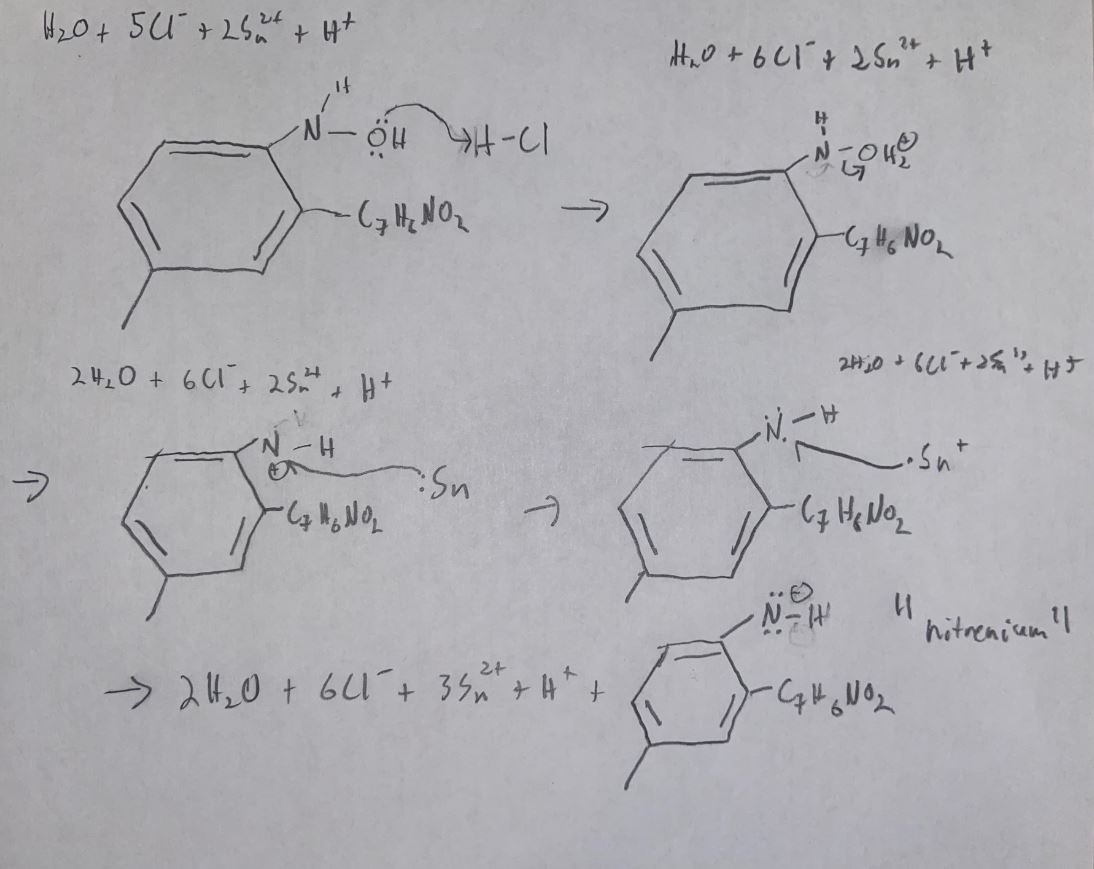
\includegraphics[scale=.35]{aromatic_nitro_reduction_four.JPG}
    \end{center}
    
    \note{
    \begin{itemize}
        \item Recall these radical attacks can happen on second go from other equivalents of Tin
        \item Nitrenium intermediate observed
    \end{itemize}}
\end{frame}

\begin{frame}{Reduction of Aromatic Nitro Groups: Mechanism \#5}
    \begin{center}
        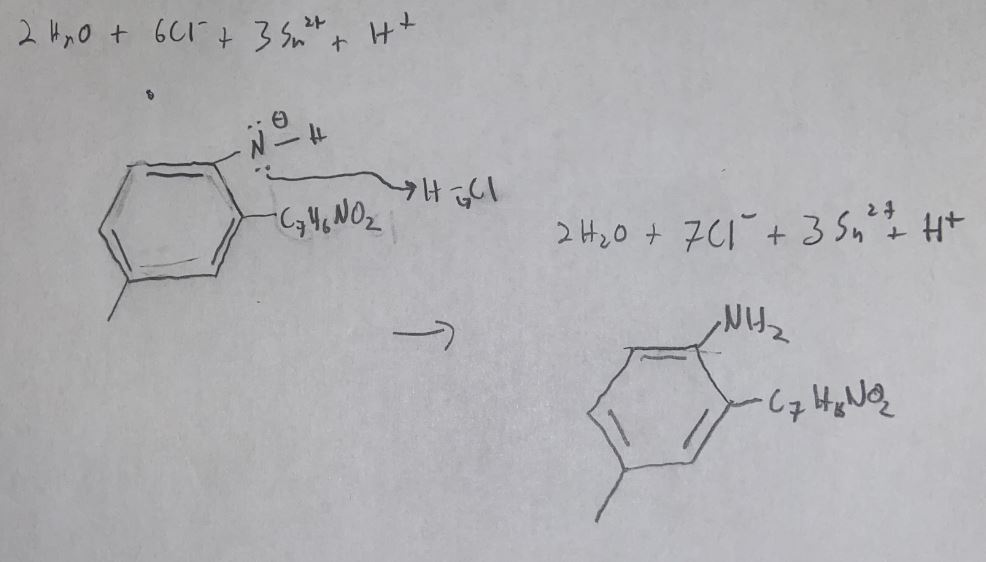
\includegraphics[scale=.4]{aromatic_nitro_reduction_five.JPG}
    \end{center}
    
    \note{
    \begin{itemize}
        \item One reduction achieved
    \end{itemize}
    }
\end{frame}

\begin{frame}{Reduction of Aromatic Nitro Groups: Mechanism \#6}
    \begin{center}
        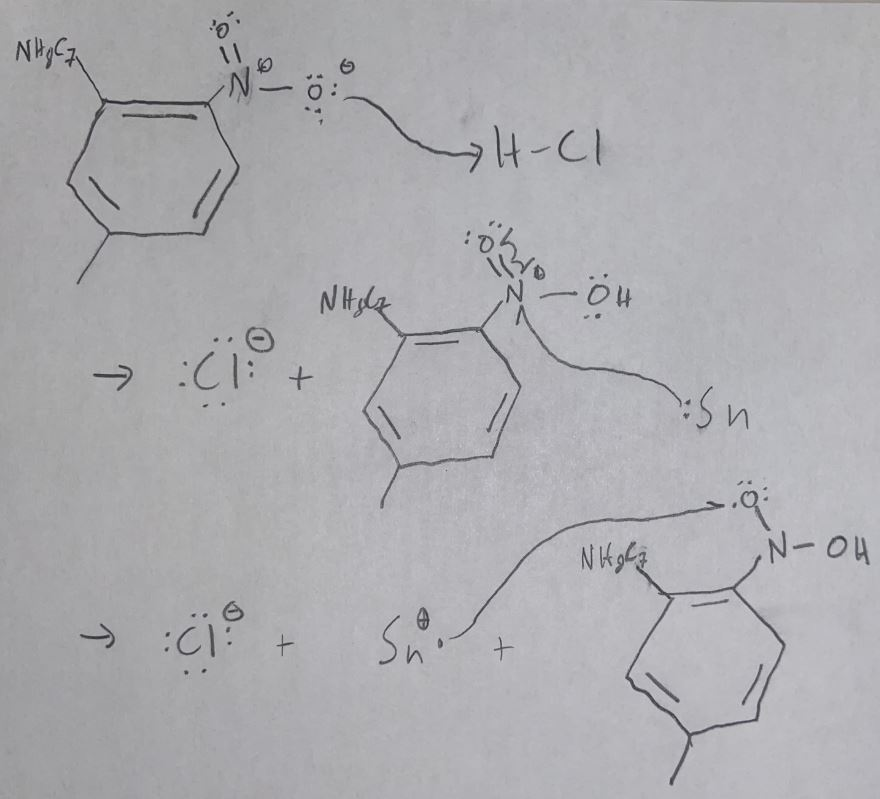
\includegraphics[scale=.35]{aromatic_nitro_reduction_six.JPG}
    \end{center}
    
    \note{
    \begin{itemize}
        \item The rest of this we'll zoom throught, it basically just happens twice.
    \end{itemize}
    }
\end{frame}

\begin{frame}{Reduction of Aromatic Nitro Groups: Mechanism \#7}
    \begin{center}
        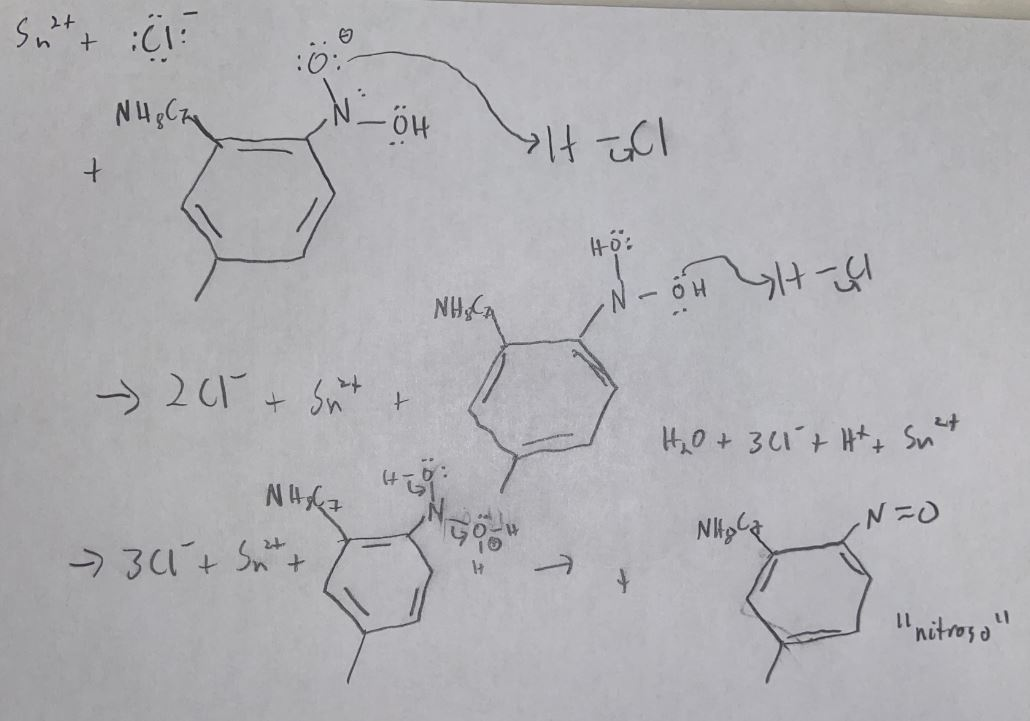
\includegraphics[scale=.4]{aromatic_nitro_reduction_seven.JPG}
    \end{center}
    
    \note{
    \begin{itemize}
        \item The rest of this we'll zoom throught, it basically just happens twice.
    \end{itemize}
    }
\end{frame}

\begin{frame}{Reduction of Aromatic Nitro Groups: Mechanism \#8}
    \begin{center}
        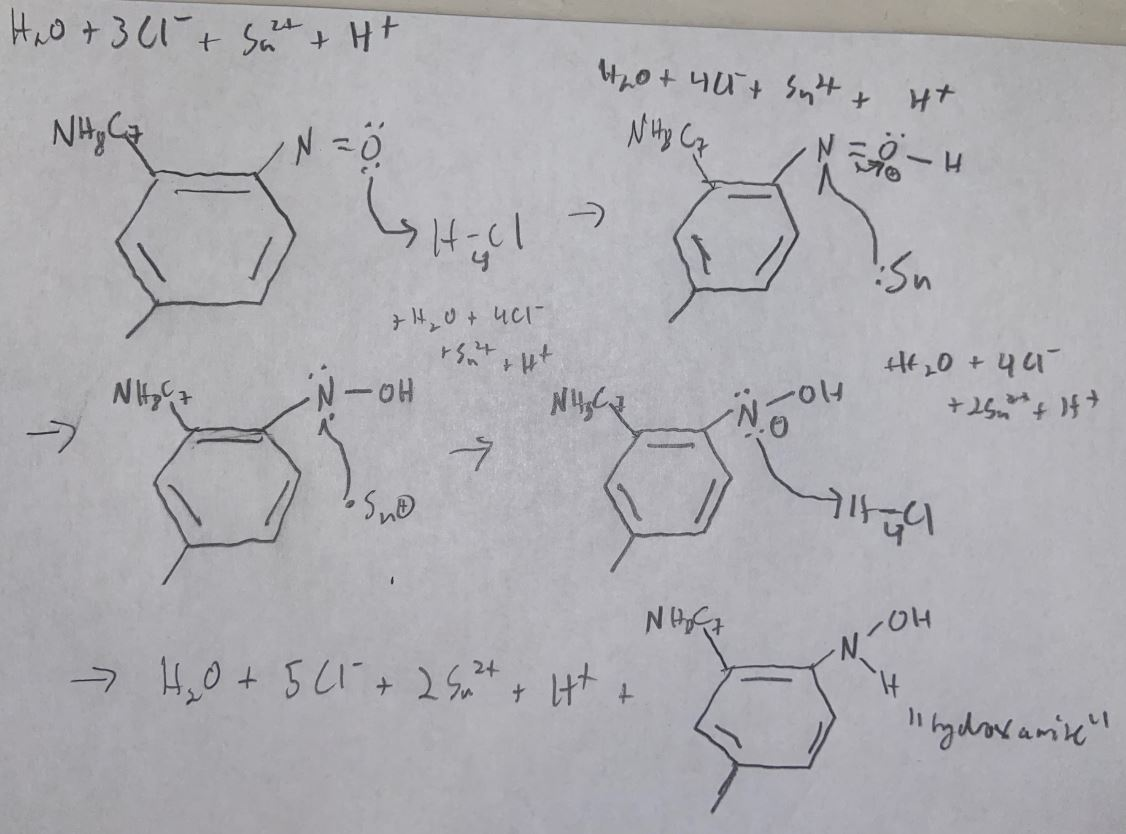
\includegraphics[scale=.32]{aromatic_nitro_reduction_eight.JPG}
    \end{center}
    
    \note{
    \begin{itemize}
        \item The rest of this we'll zoom throught, it basically just happens twice.
    \end{itemize}
    }
\end{frame}

\begin{frame}{Reduction of Aromatic Nitro Groups: Mechanism \#9}
    \begin{center}
        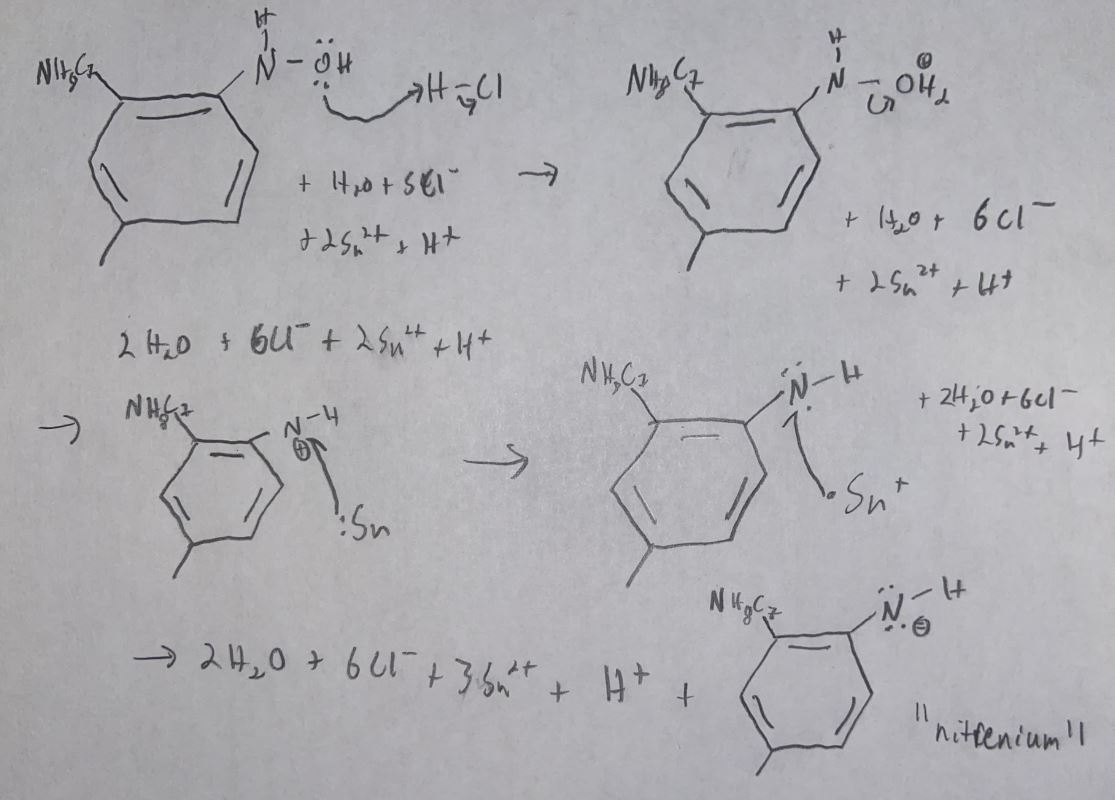
\includegraphics[scale=.32]{aromatic_nitro_reduction_nine.JPG}
    \end{center}
    
    \note{
    \begin{itemize}
        \item The rest of this we'll zoom throught, it basically just happens twice.
    \end{itemize}
    }
\end{frame}

\begin{frame}{Reduction of Aromatic Nitro Groups: Mechanism \#10}
    \begin{center}
        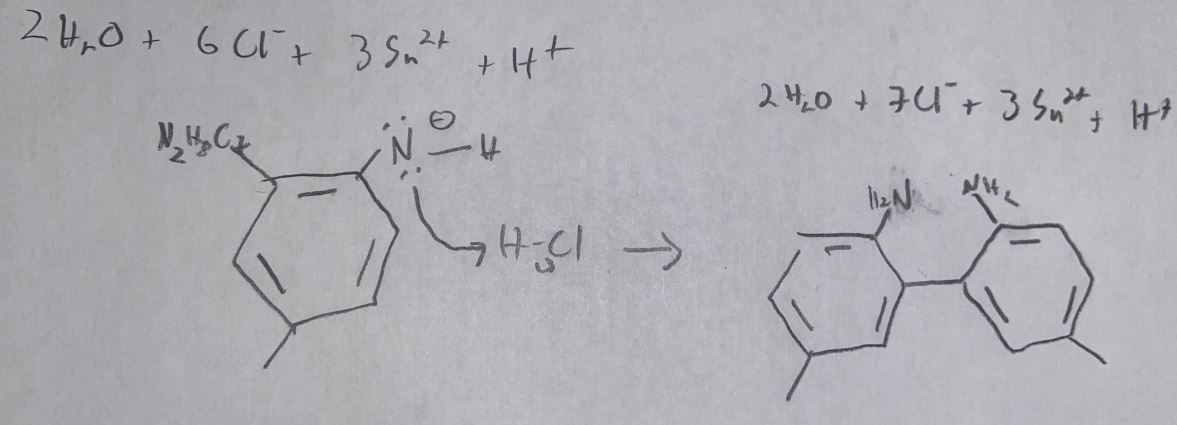
\includegraphics[scale=.3]{aromatic_nitro_reduction_ten.JPG}
    \end{center}
    
    \note{
    \begin{itemize}
        \item The rest of this we'll zoom throught, it basically just happens twice.
    \end{itemize}
    }
\end{frame}

\begin{frame}{Sandmeyer Reaction Part One}

\begin{center}
    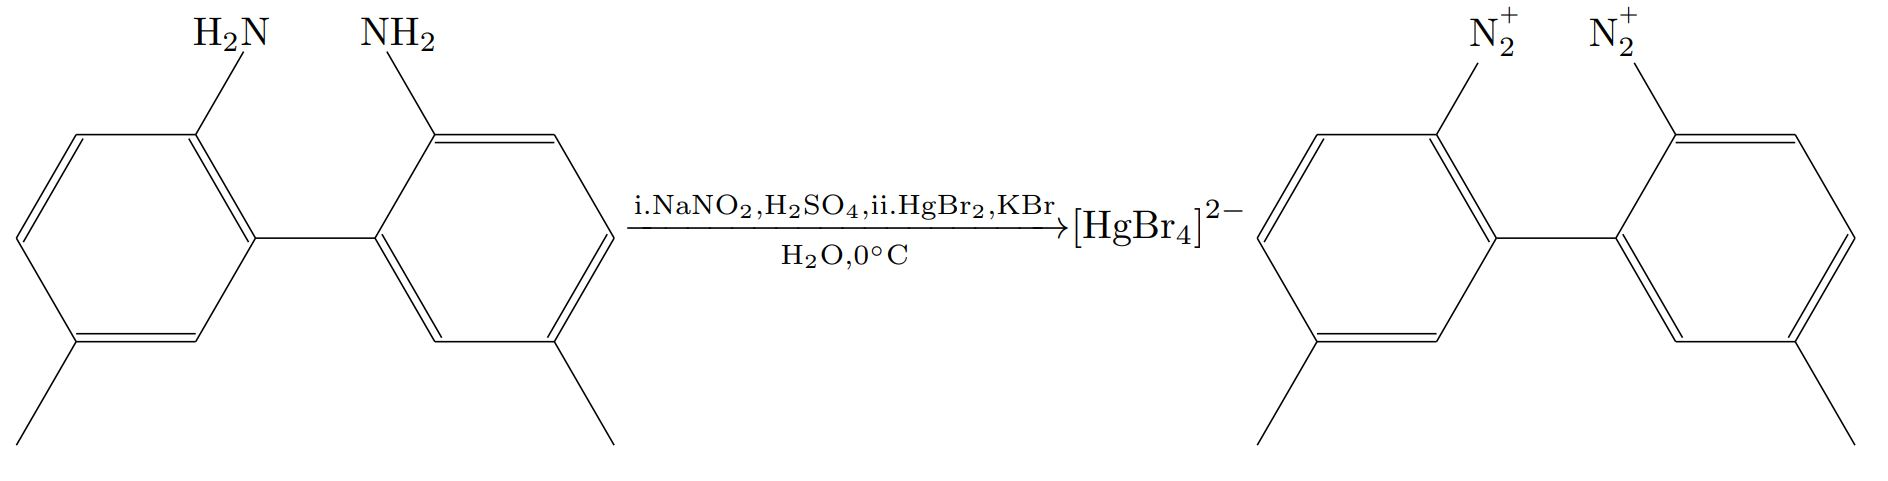
\includegraphics[scale=.22]{sandmeyer_part_one_overall.JPG}
\end{center}
\note{\begin{itemize}
    \item \cite{Beaudoin} is the source for both this reaction and the next one. 
    \item It's another key SET mechanism in the second part
\end{itemize}}
    
\end{frame}

\begin{frame}{Sandmeyer Reaction Part One: Mechanism \#1}

\begin{center}
    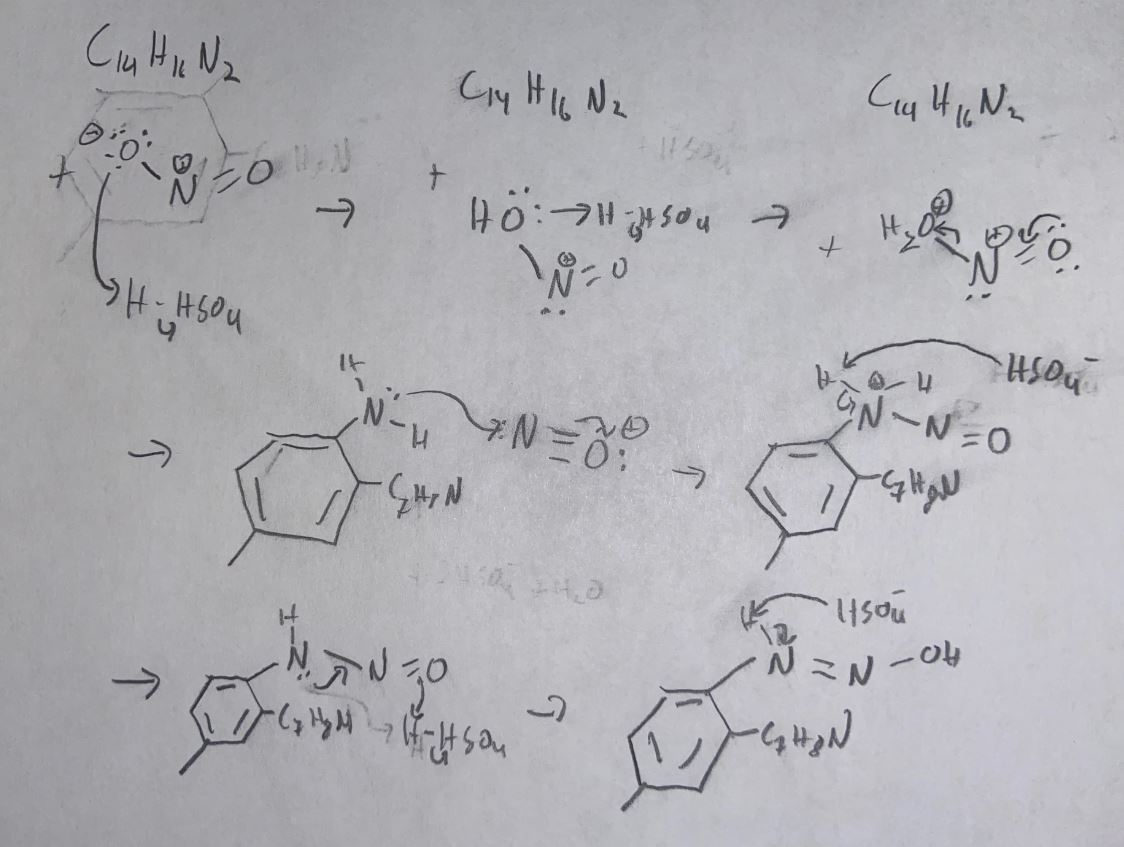
\includegraphics[scale=.35]{sandmeyer_part_one_one.JPG}
\end{center}

\note{\begin{itemize}
    \item Note \mathrm{HSO_4^{-}} as amphiprotic is at play.
\end{itemize}}
    
\end{frame}

\begin{frame}{Sandmeyer Reaction Part One: Mechanism \#2}

\begin{center}
    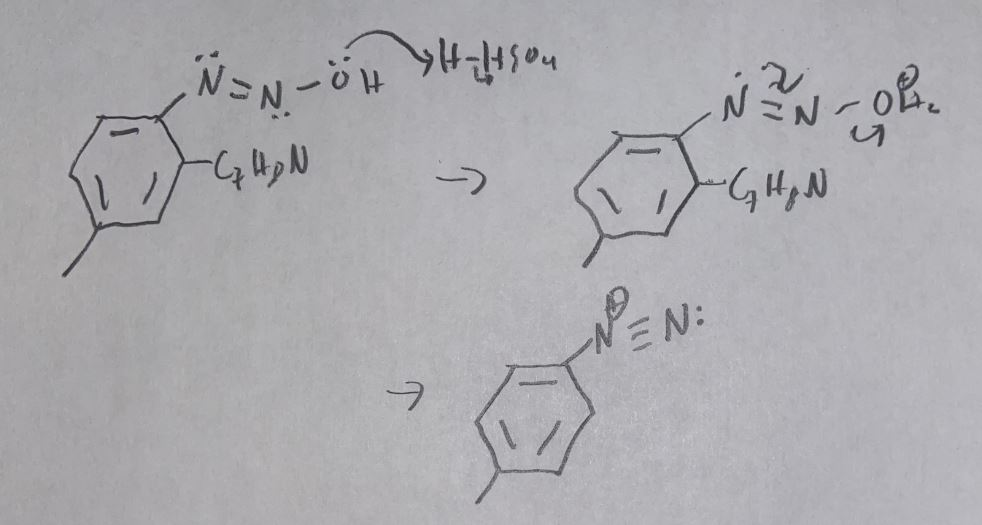
\includegraphics[scale=.38]{sandmeyer_part_one_two.JPG}
\end{center}

\note{\begin{itemize}
    \item Water production a driving force
    \item More substituted amino cation more stable.
\end{itemize}}
    
\end{frame}

\begin{frame}{Sandmeyer Reaction Part One: Mechanism \#3}

\begin{center}
    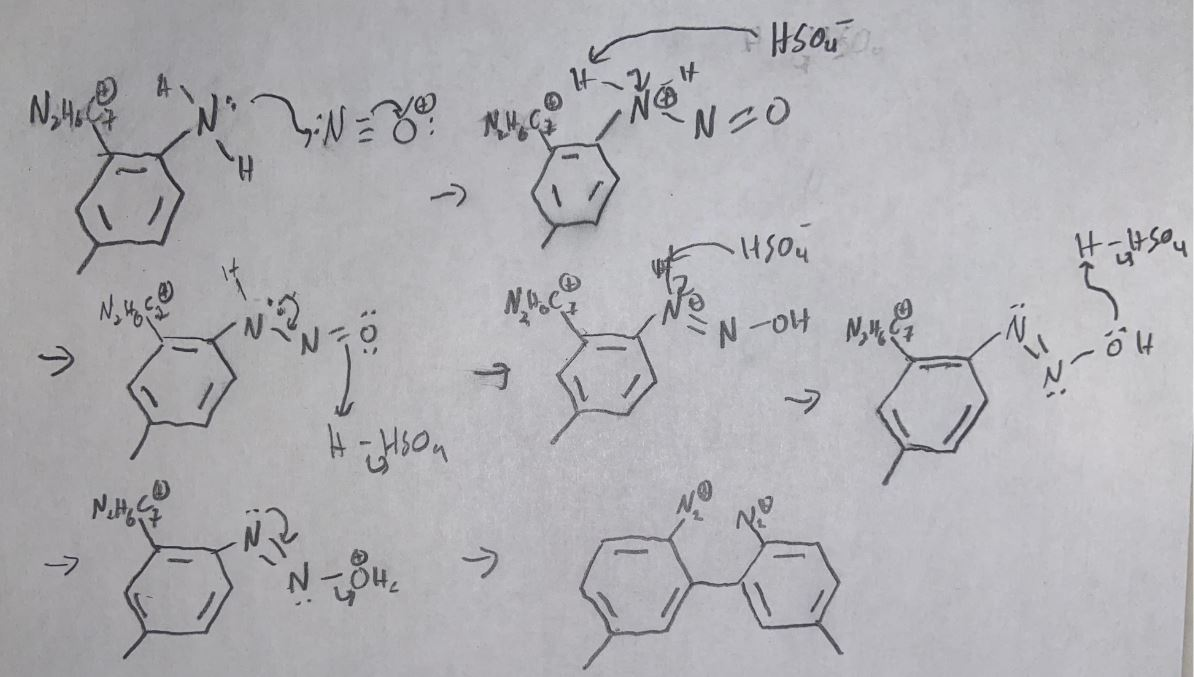
\includegraphics[scale=.35]{sandmeyer_part_one_three.JPG}
\end{center}

\note{\begin{itemize}
    \item 
\end{itemize}}
    
\end{frame}

\begin{frame}{Sandmeyer Reaction Part Two}
    \begin{center}
        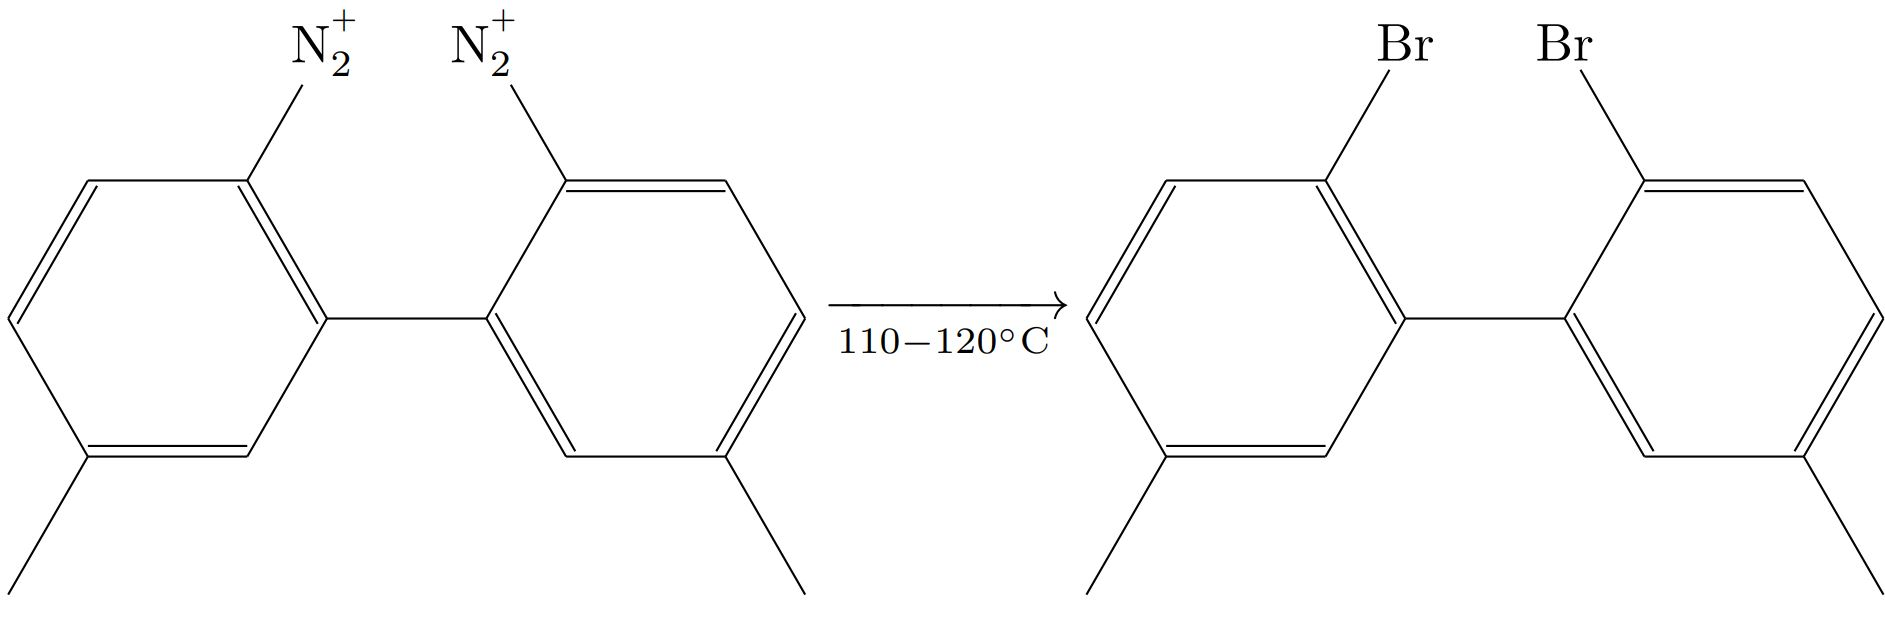
\includegraphics[scale=.2]{sandmeyer_part_two_overall.JPG}
    \end{center}
    
    \note{\begin{itemize}
        \item Driving force is production of Nitrogen gas.
        \item I'm also going to stop copying over my paper notes here. I think I'm just kind of wasting my time. 
    \end{itemize}}
\end{frame}

\begin{frame}{Sandmeyer Reaction Part Two: Mechanism \#1}

\begin{center}
    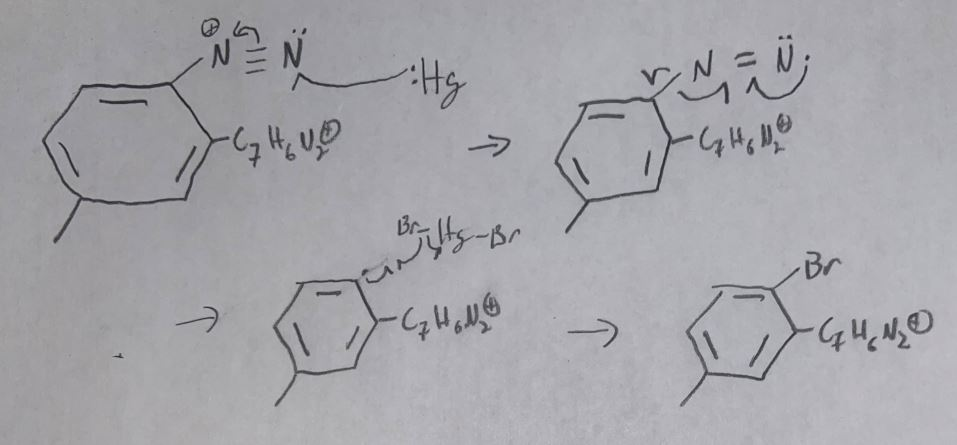
\includegraphics[scale = .39]{sandmeyer_part_two_one.JPG}
\end{center}
    
    \note{\begin{itemize}
    \item 
\end{itemize}}

\end{frame}

\begin{frame}{Sandmeyer Reaction Part Two: Mechanism \#2}

\begin{center}
    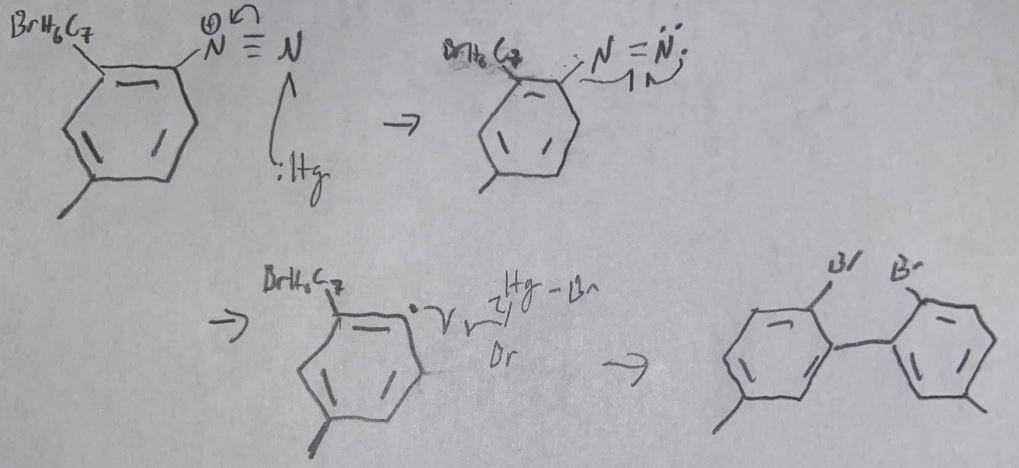
\includegraphics[scale = .382]{sandmeyer_part_two_two.JPG}
\end{center}
    
    \note{\begin{itemize}
    \item 
\end{itemize}}

\end{frame}

\begin{frame}{Wohl-Ziegler Reaction}

\begin{center}
    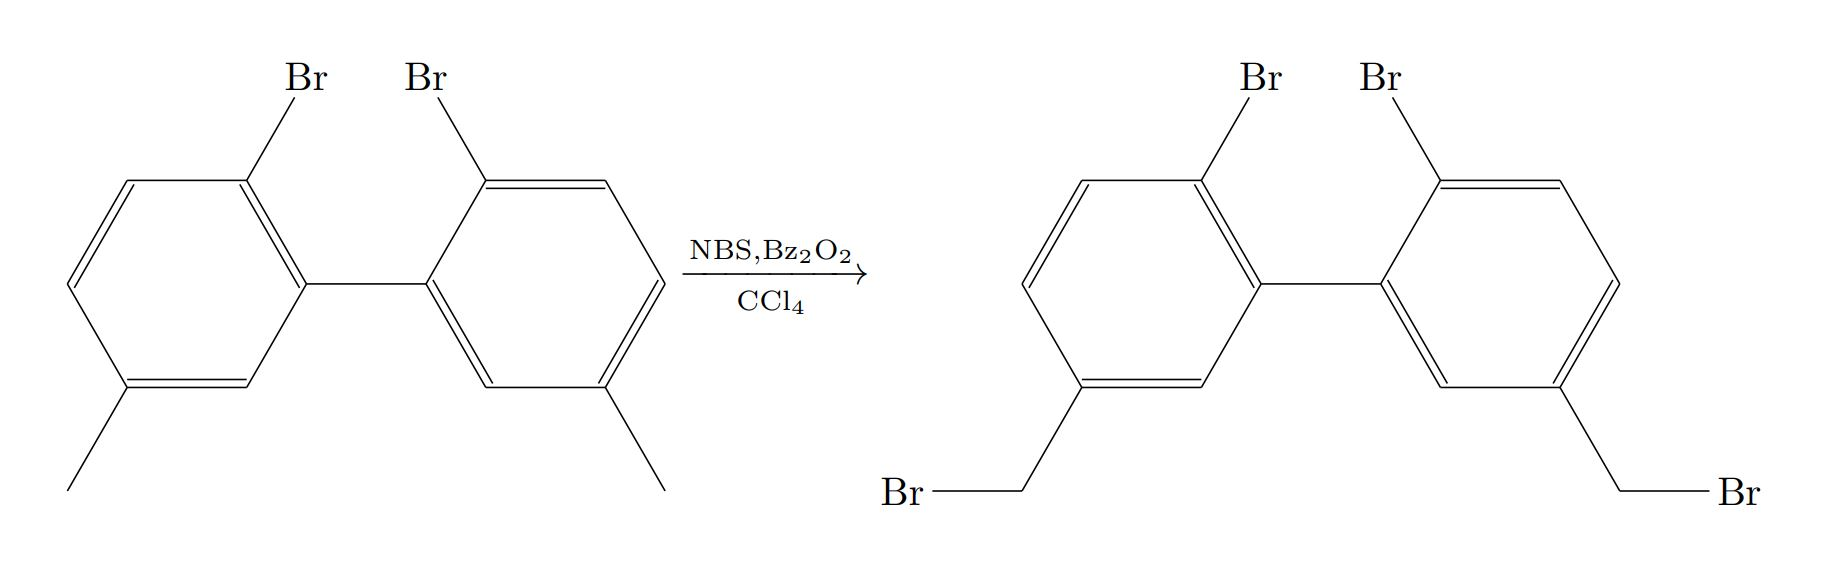
\includegraphics[scale=.2]{wohl_ziegler_overall.JPG}
\end{center}
    
\note{\begin{itemize}
    \item This is the standard radical halogenation of alkanes we learned in august.
\end{itemize}}

\end{frame}

\begin{frame}{Wohl-Ziegler Reaction: Mechanism \#1}

\begin{center}
    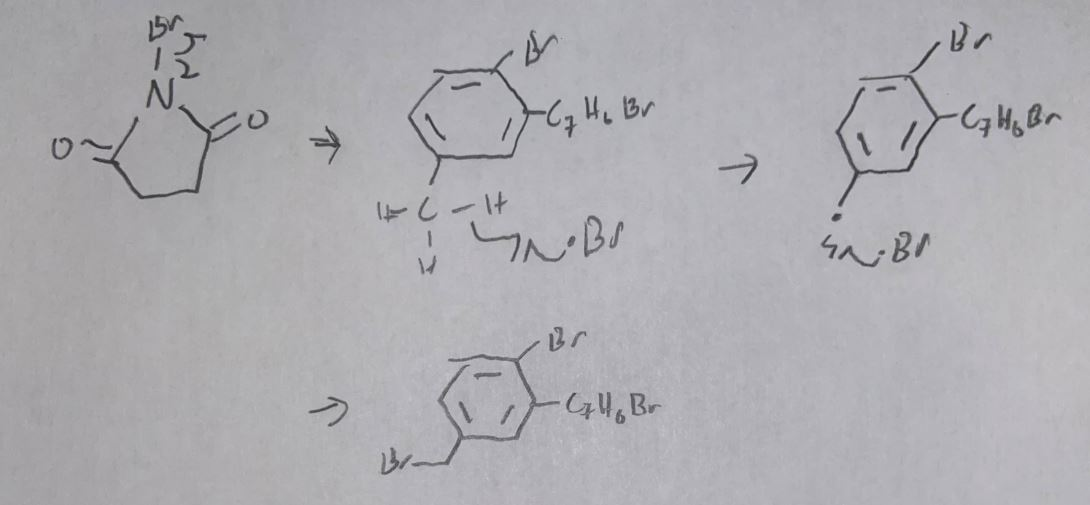
\includegraphics[scale=.35]{wohl_ziegler_one.JPG}
\end{center}
    
\note{\begin{itemize}
    \item 
\end{itemize}}

\end{frame}

\begin{frame}{Wohl-Ziegler Reaction: Mechanism \#2}

\begin{center}
    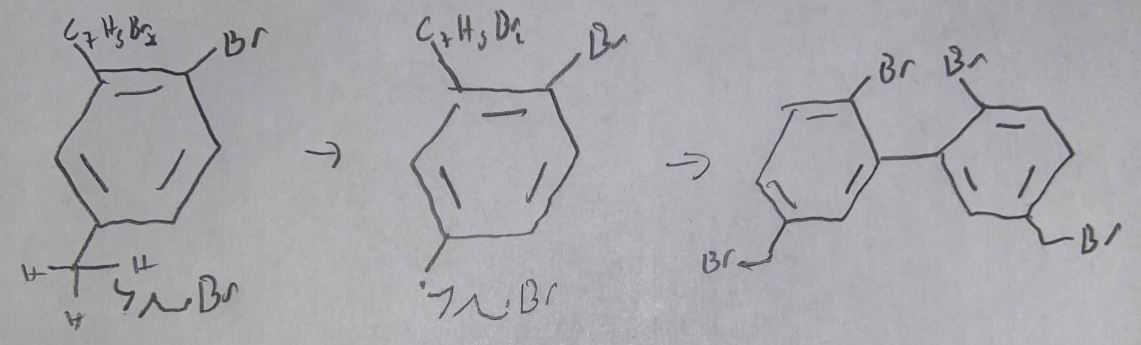
\includegraphics[scale=.35]{wohl_ziegler_two.JPG}
\end{center}
    
\note{\begin{itemize}
    \item 
\end{itemize}}

\end{frame}

\begin{frame}{Thiolization Part One}
\begin{center}
    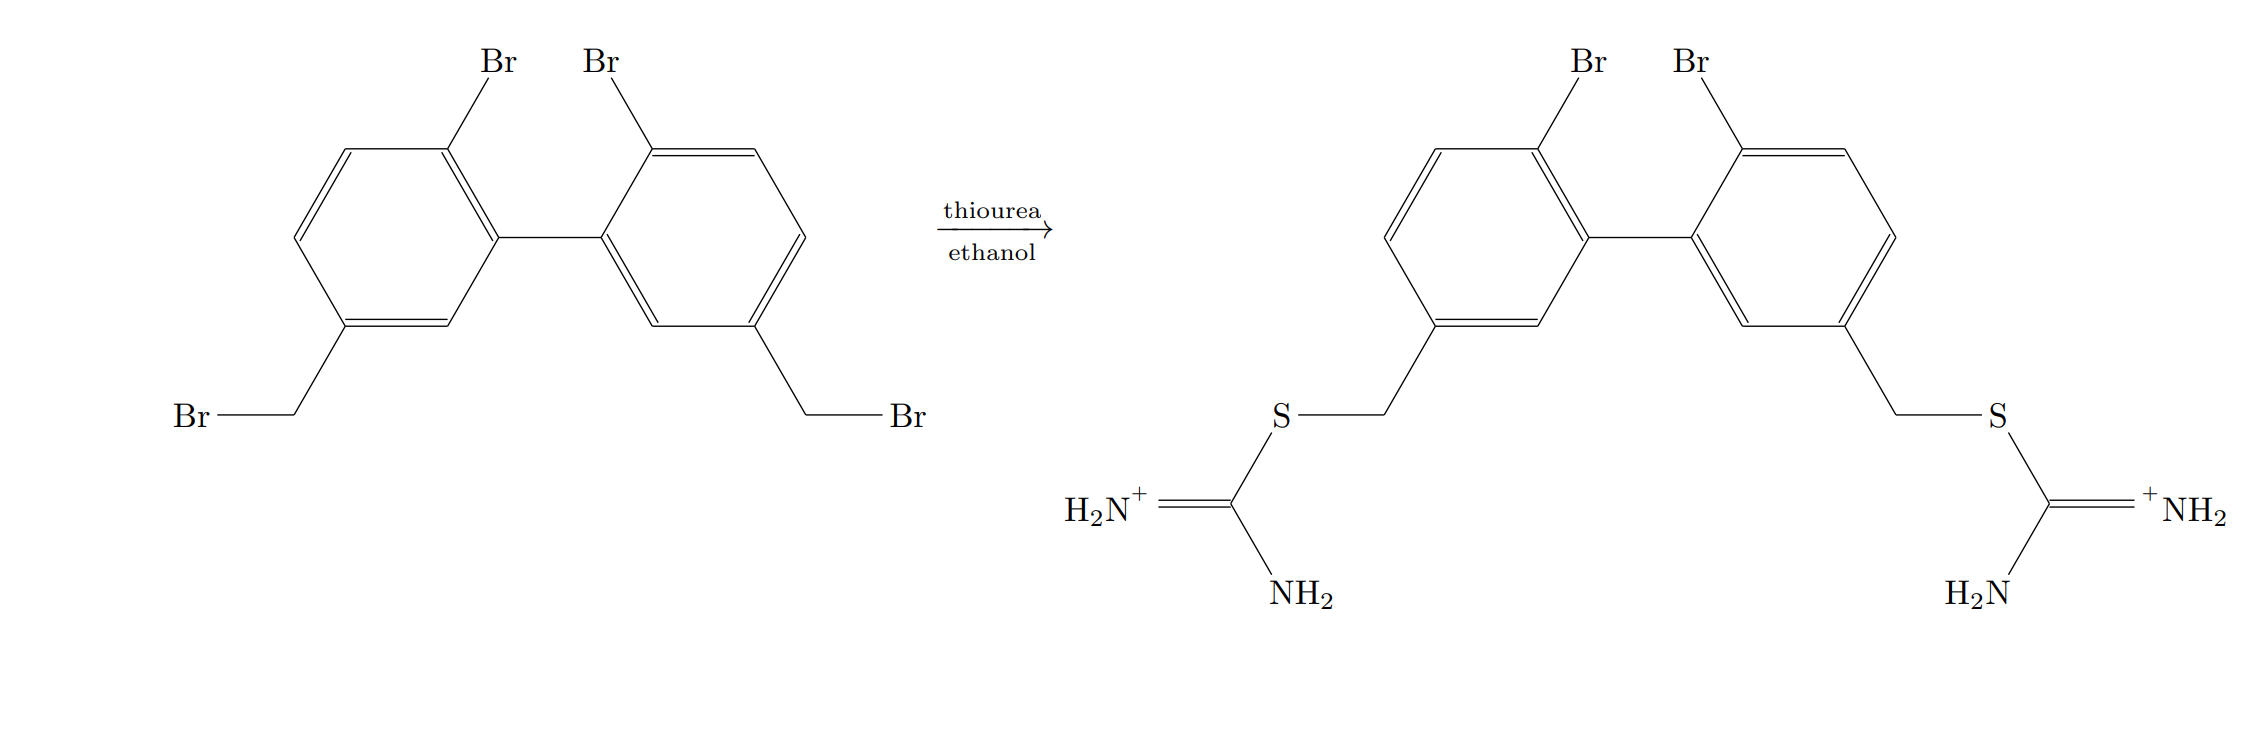
\includegraphics[scale=.4]{thiolization_part_one_overall.PNG}
\end{center}
\end{frame}

\begin{frame}{Thiolization Part One: Mechanism \#1}
\begin{center}
    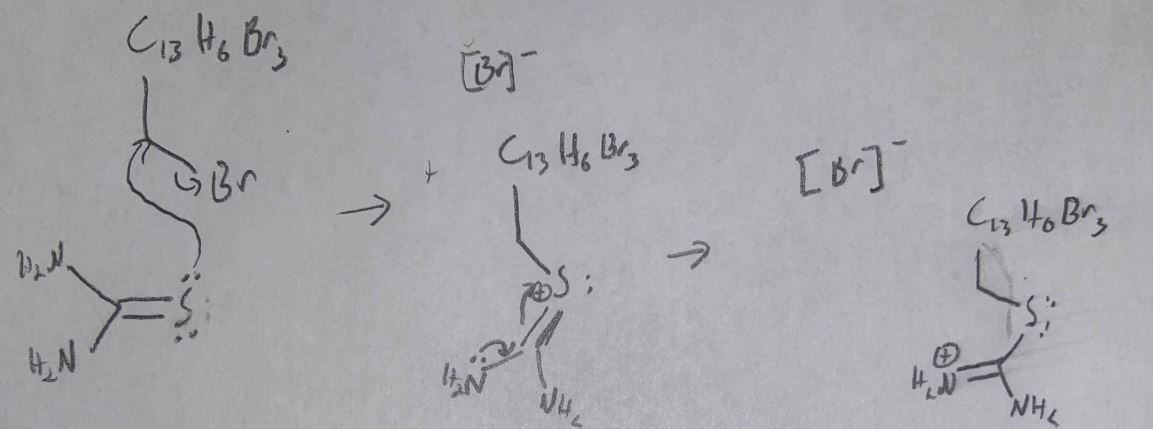
\includegraphics[scale=.4]{thiolization_part_one_one.JPG}
\end{center}
\end{frame}

\begin{frame}{Thiolization Part One: Mechanism \#2}
\begin{center}
    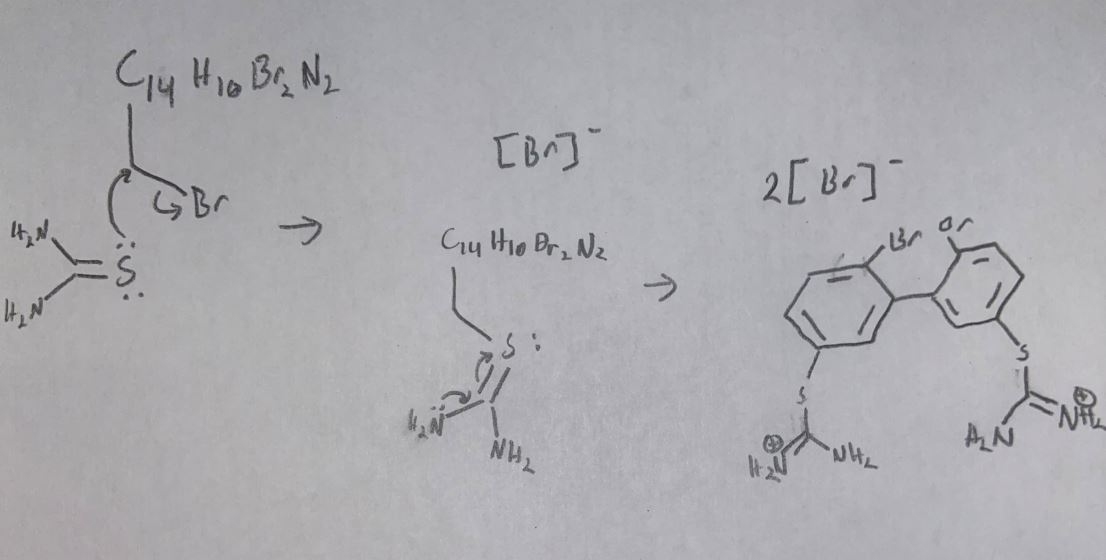
\includegraphics[scale=.4]{thiolization_part_one_two.JPG}
\end{center}
\end{frame}

\begin{frame}{Thiolization Part Two}
\begin{center}
    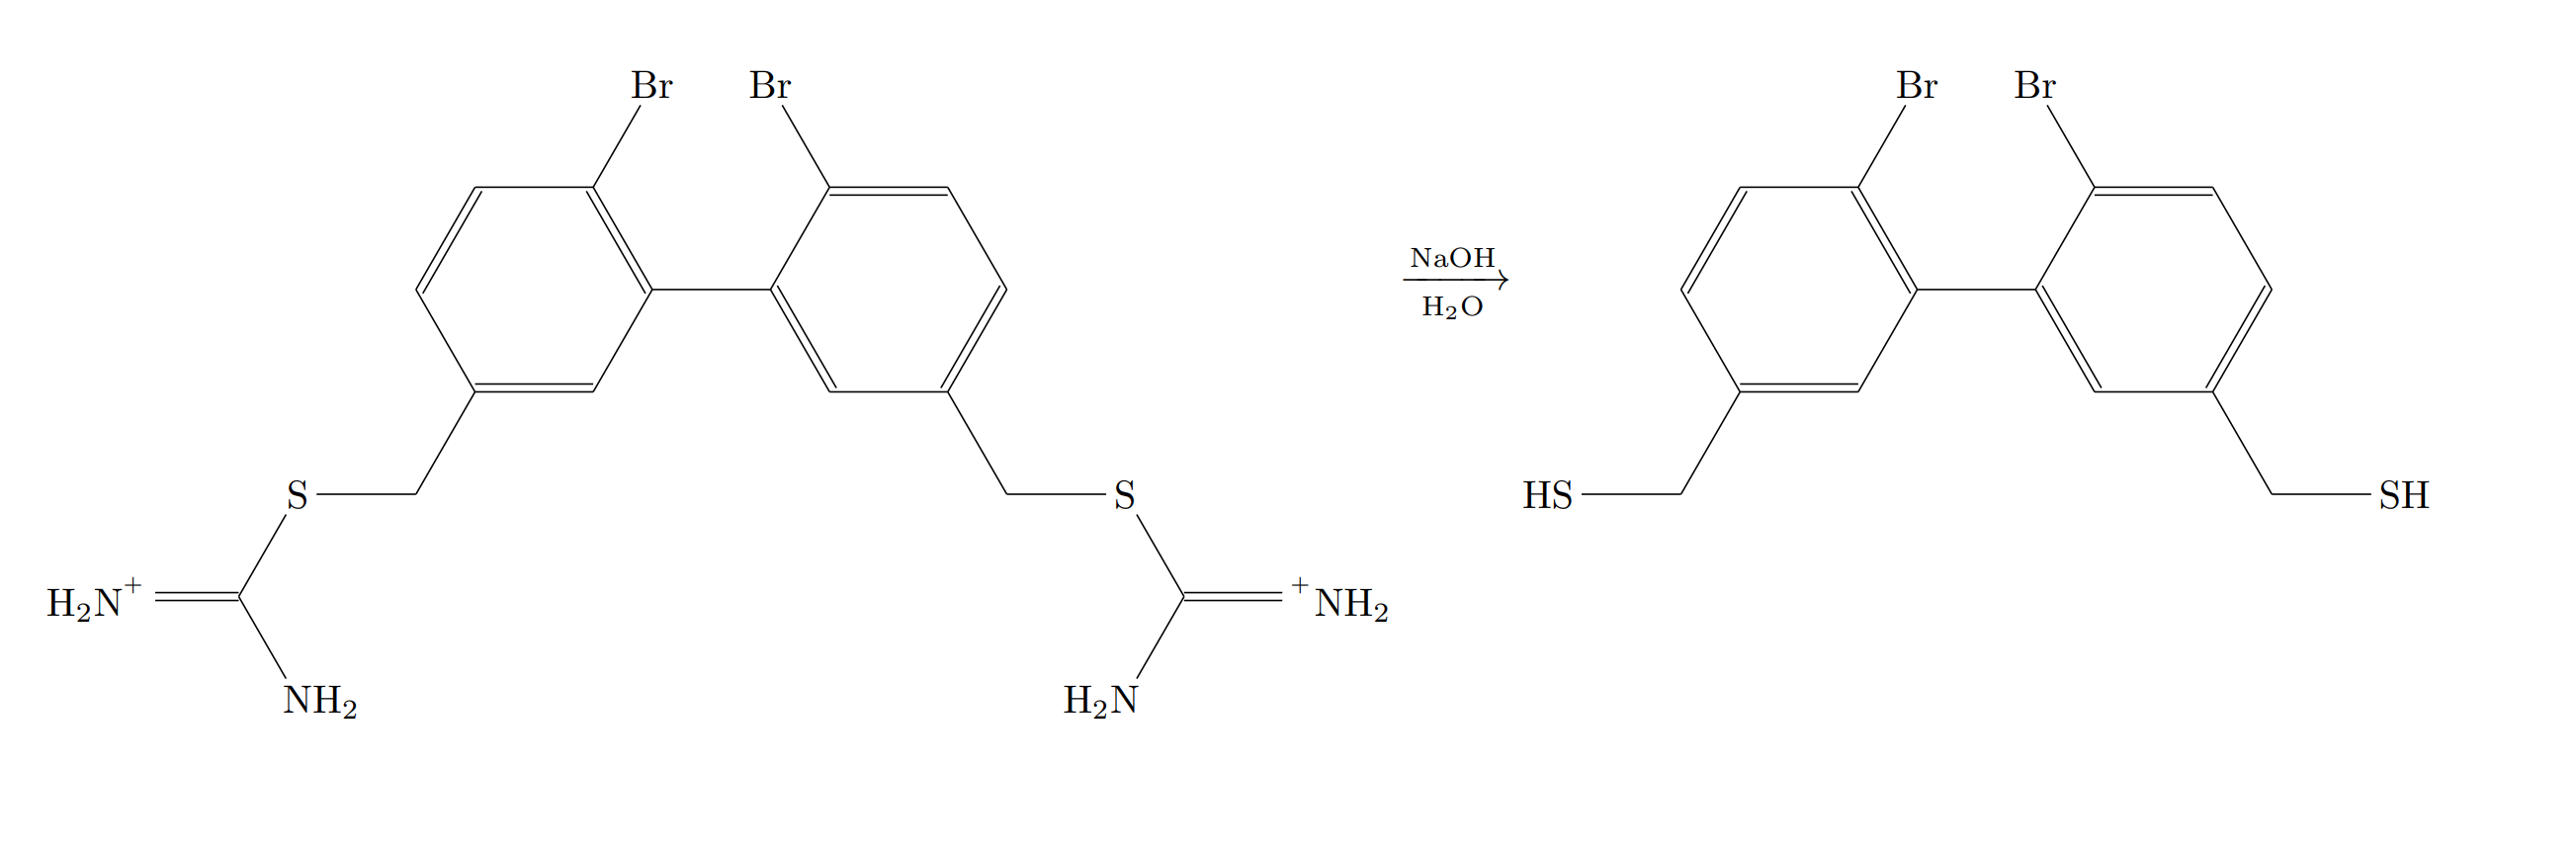
\includegraphics[scale=.35]{thiolization_part_two_overall.PNG}
\end{center}
\end{frame}

\begin{frame}{Thiolization Part Two: Mechanism \#1}
\begin{center}
    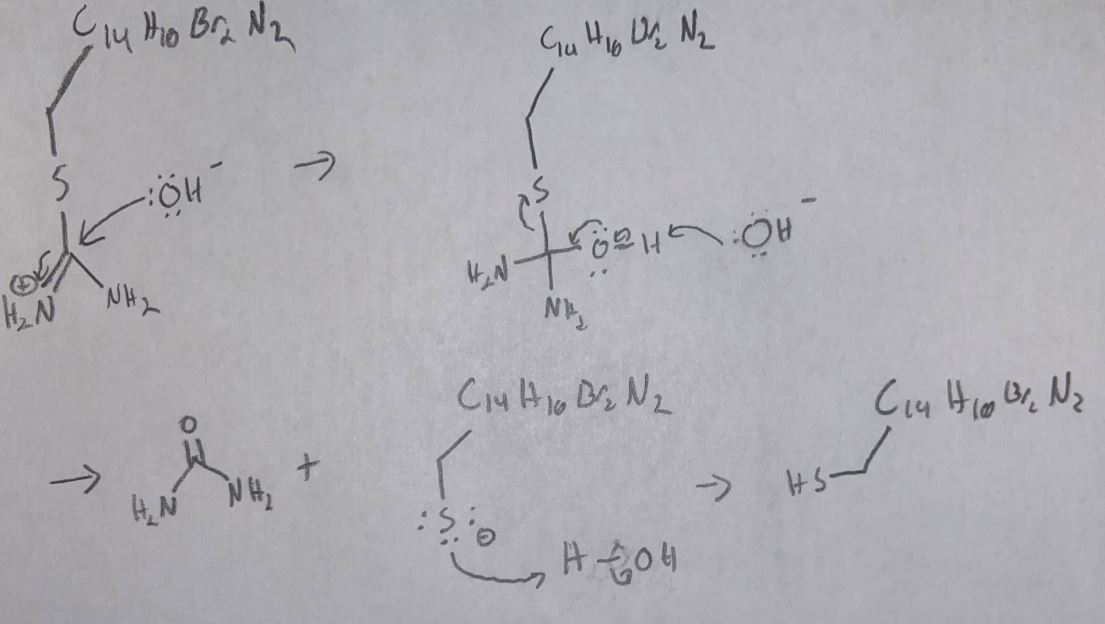
\includegraphics[scale=.4]{thiolization_part_two_one.JPG}
\end{center}
\end{frame}

\begin{frame}{Thiolization Part Two: Mechanism \#2}
\begin{center}
    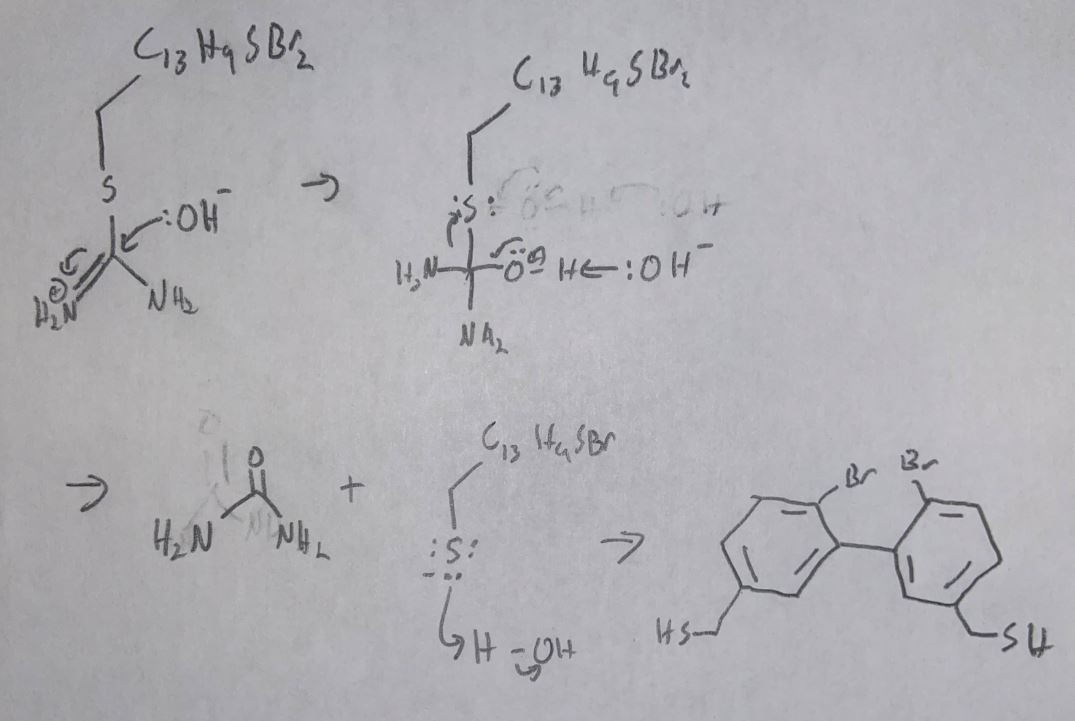
\includegraphics[scale=.4]{thiolization_part_two_two.JPG}
\end{center}
\end{frame}



\begin{frame}{Williamson Thioether Synthesis}
\begin{center}
    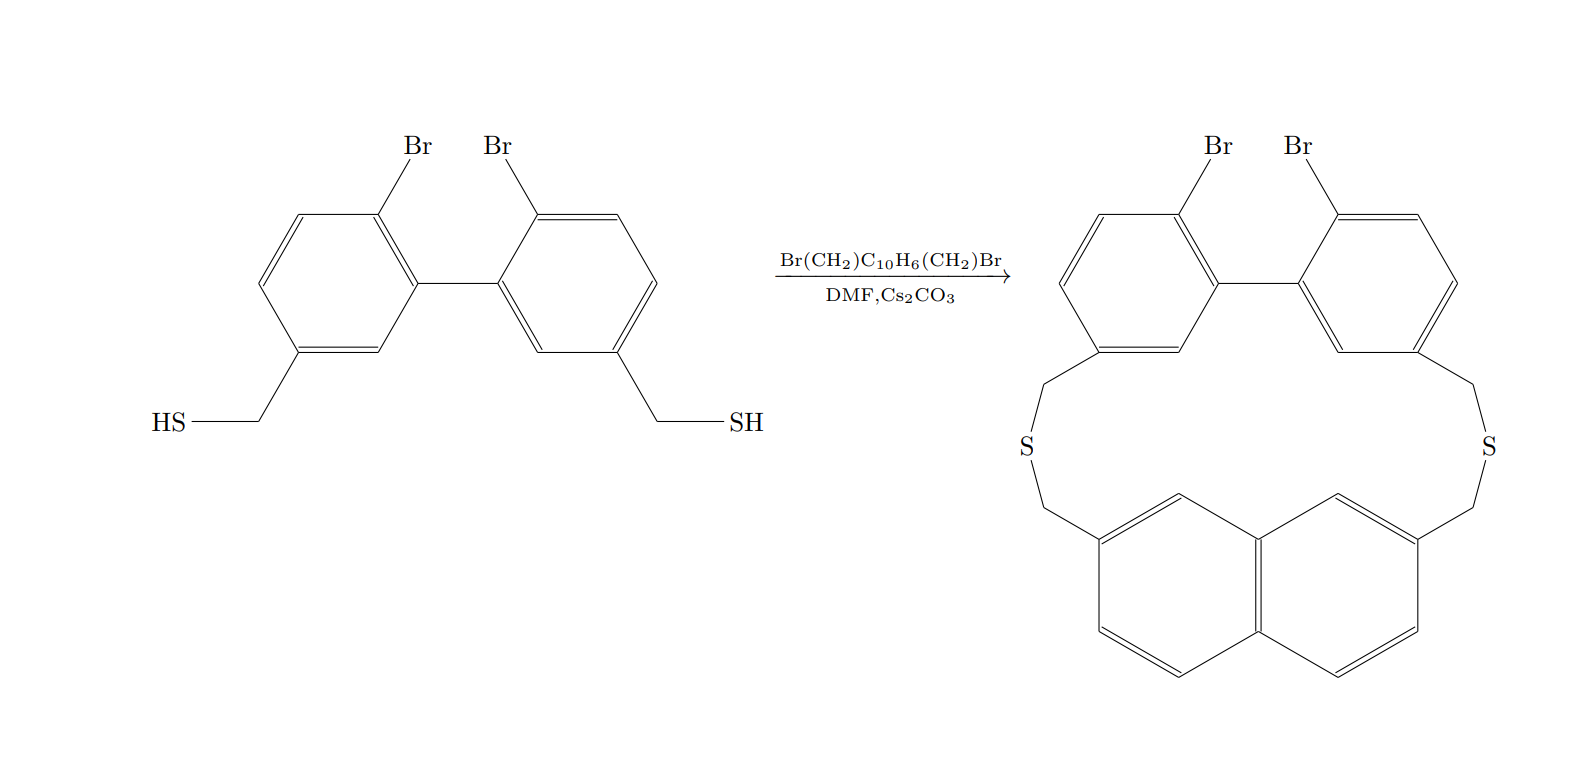
\includegraphics[scale=.4]{williamson_thioether_synthesis_overall.PNG}
\end{center}
\end{frame}

\begin{frame}{Williamson Thioether Synthesis: Mechanism \#1}
\begin{center}
    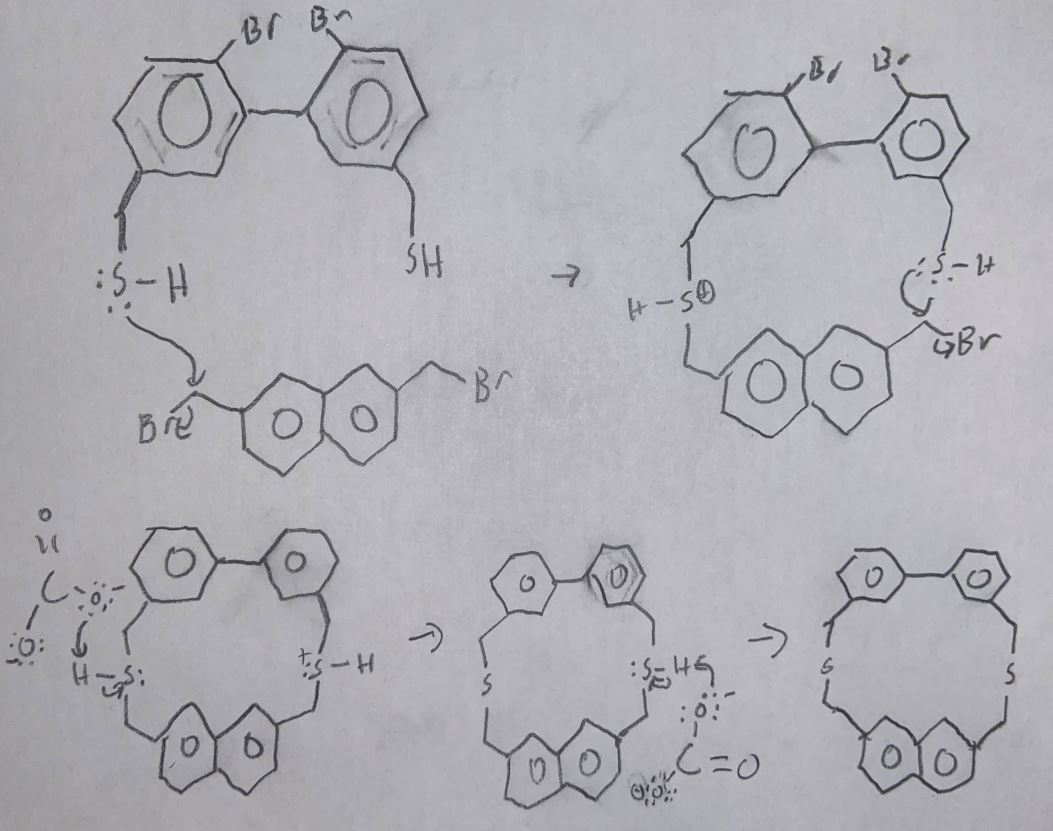
\includegraphics[scale=.35]{williamson_thioether_synthesis_one.JPG}
\end{center}
\end{frame}


\begin{frame}{Thioether Methylation}
\begin{center}
    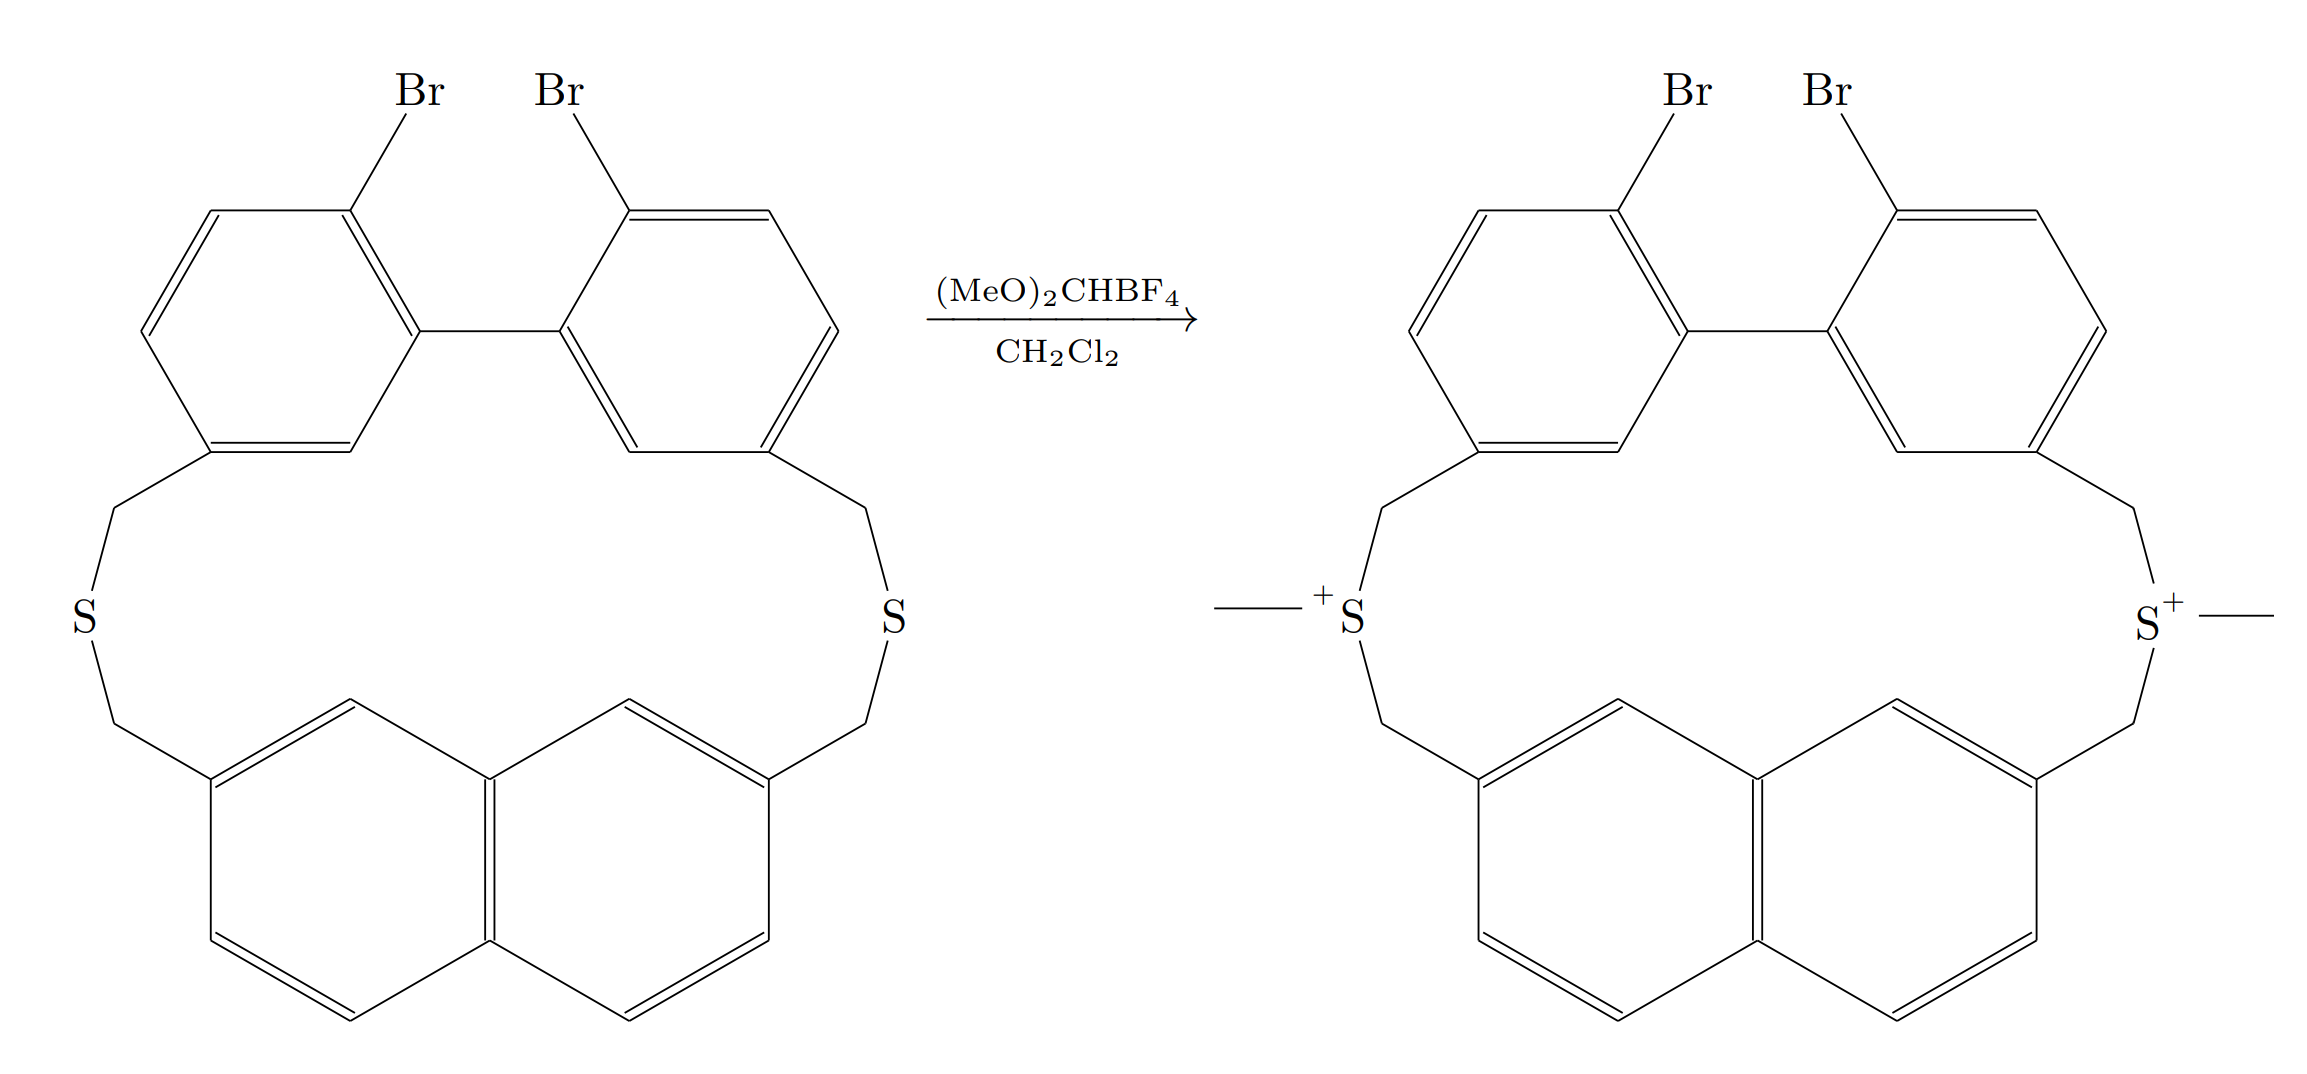
\includegraphics[scale=.4]{thioether_methylation_overall.PNG}
\end{center}
\end{frame}

\begin{frame}{Thioether Methylation: Mechanism \#1}
\begin{center}
    \includegraphics[scale=.3]{thioether_methylation_one.JPG}
\end{center}
\end{frame}

\begin{frame}{Thioether Methylation: Mechanism \#2}
\begin{center}
    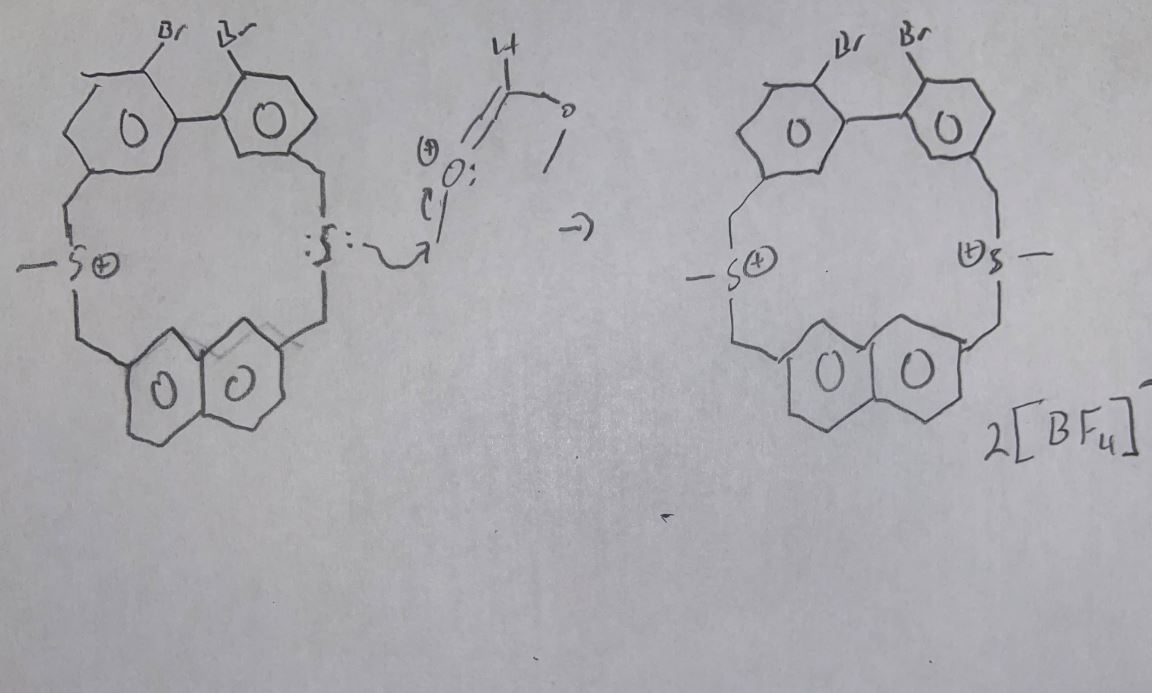
\includegraphics[scale=.4]{Thioether_methylation_Two.JPG}
\end{center}
\end{frame}

\begin{frame}{Stevens Rearrangement}
\begin{center}
    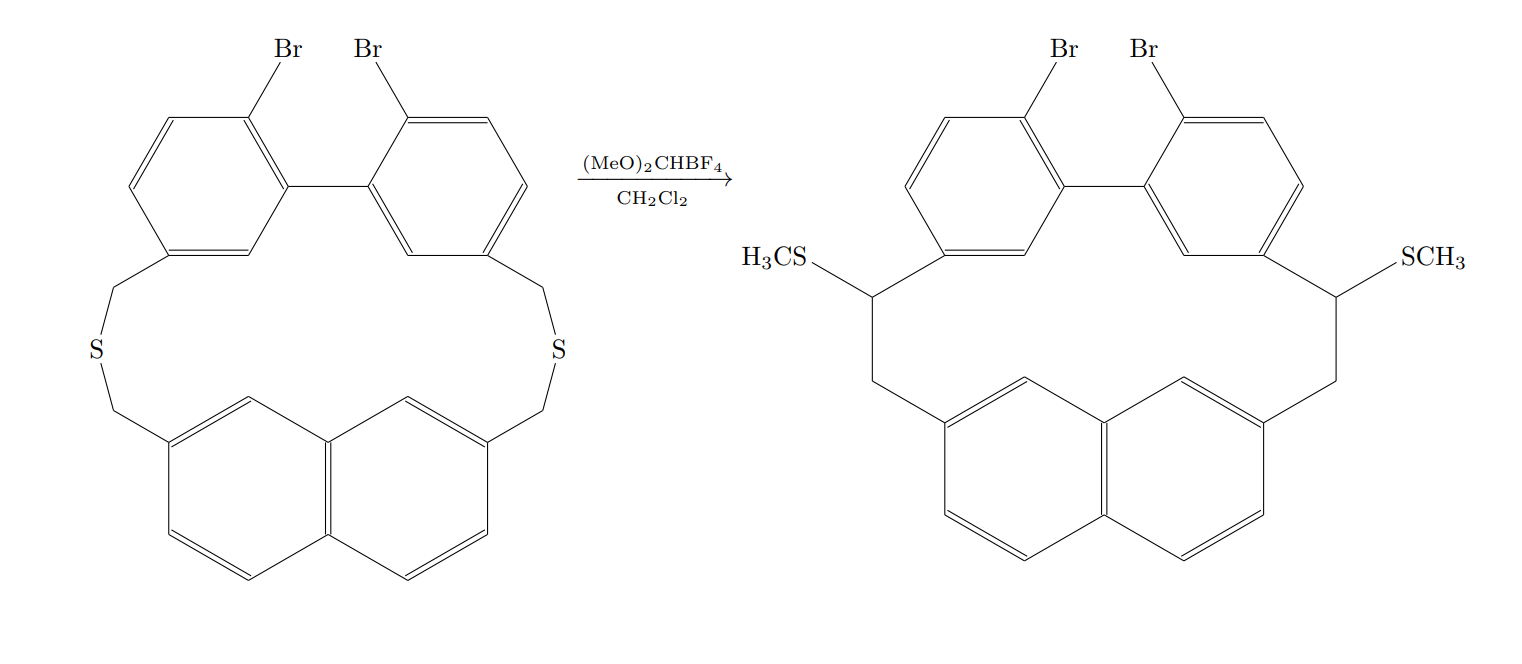
\includegraphics[scale=.46]{stevens_rearrangement_overall.PNG}
\end{center}
\end{frame}

\begin{frame}{Stevens Rearrangement: Mechanism \#1}
\begin{center}
    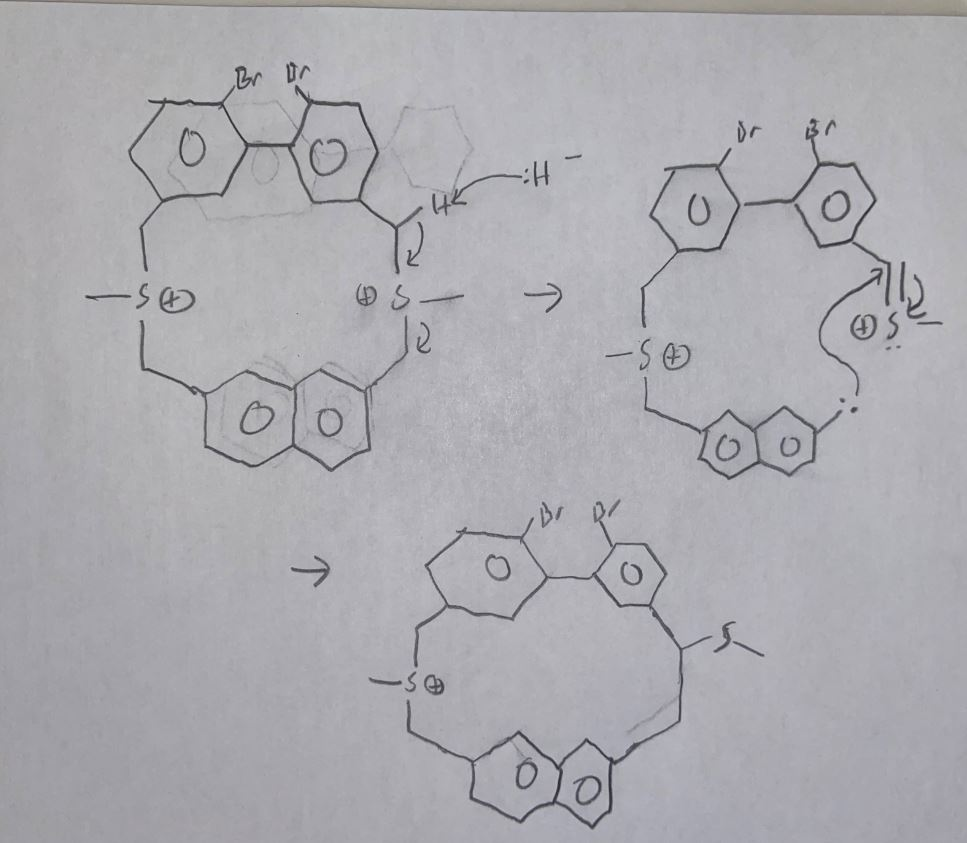
\includegraphics[scale=.32]{stevens_rearrangement_one.JPG}
\end{center}
\end{frame}

\begin{frame}{Stevens Rearrangement: Mechanism \#2}
\begin{center}
    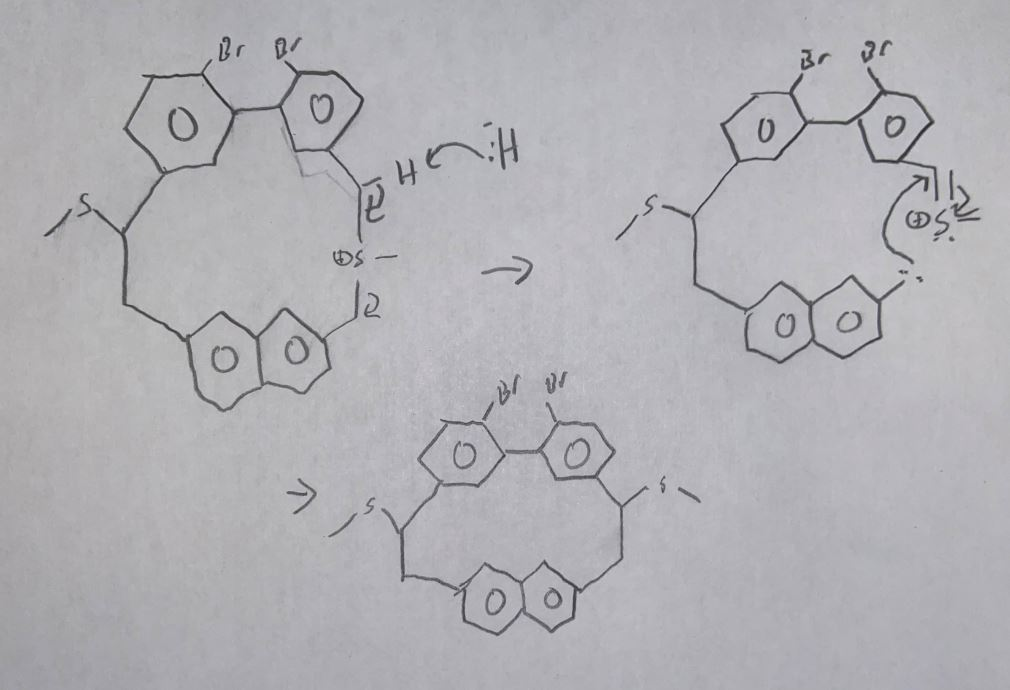
\includegraphics[scale=.37]{stevens_rearrangement_Two.JPG}
\end{center}
\end{frame}

\begin{frame}{Sulfenic Ester Tautometerization}
\begin{center}
    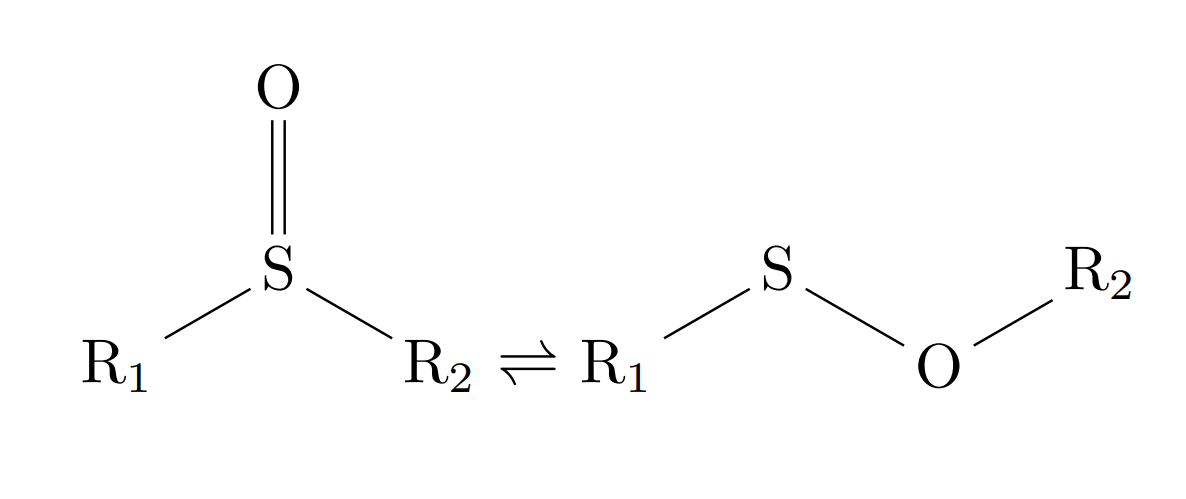
\includegraphics[scale=.52]{sulfenic_ester_tautometerization_overall.PNG}
\end{center}
\end{frame}

\begin{frame}{Sulfenic Ester Tautometerization: Mechanism \#1}
\begin{center}
    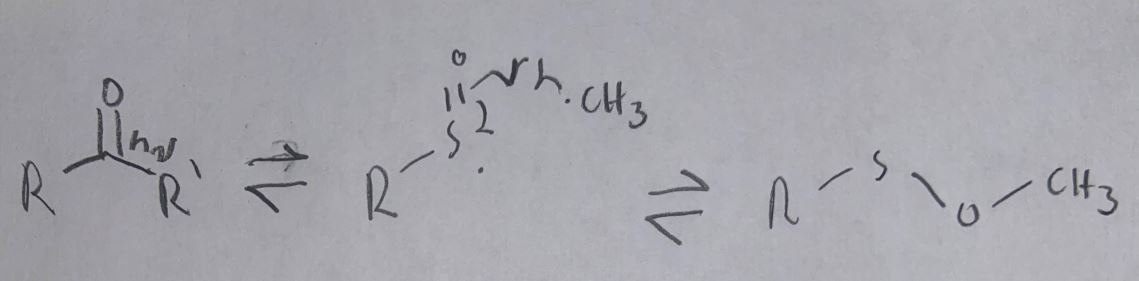
\includegraphics[scale=.32]{sulfenic_ester_tautomerization_one.JPG}
\end{center}
\end{frame}

\begin{frame}{Thioether Oxidation}
\begin{center}
    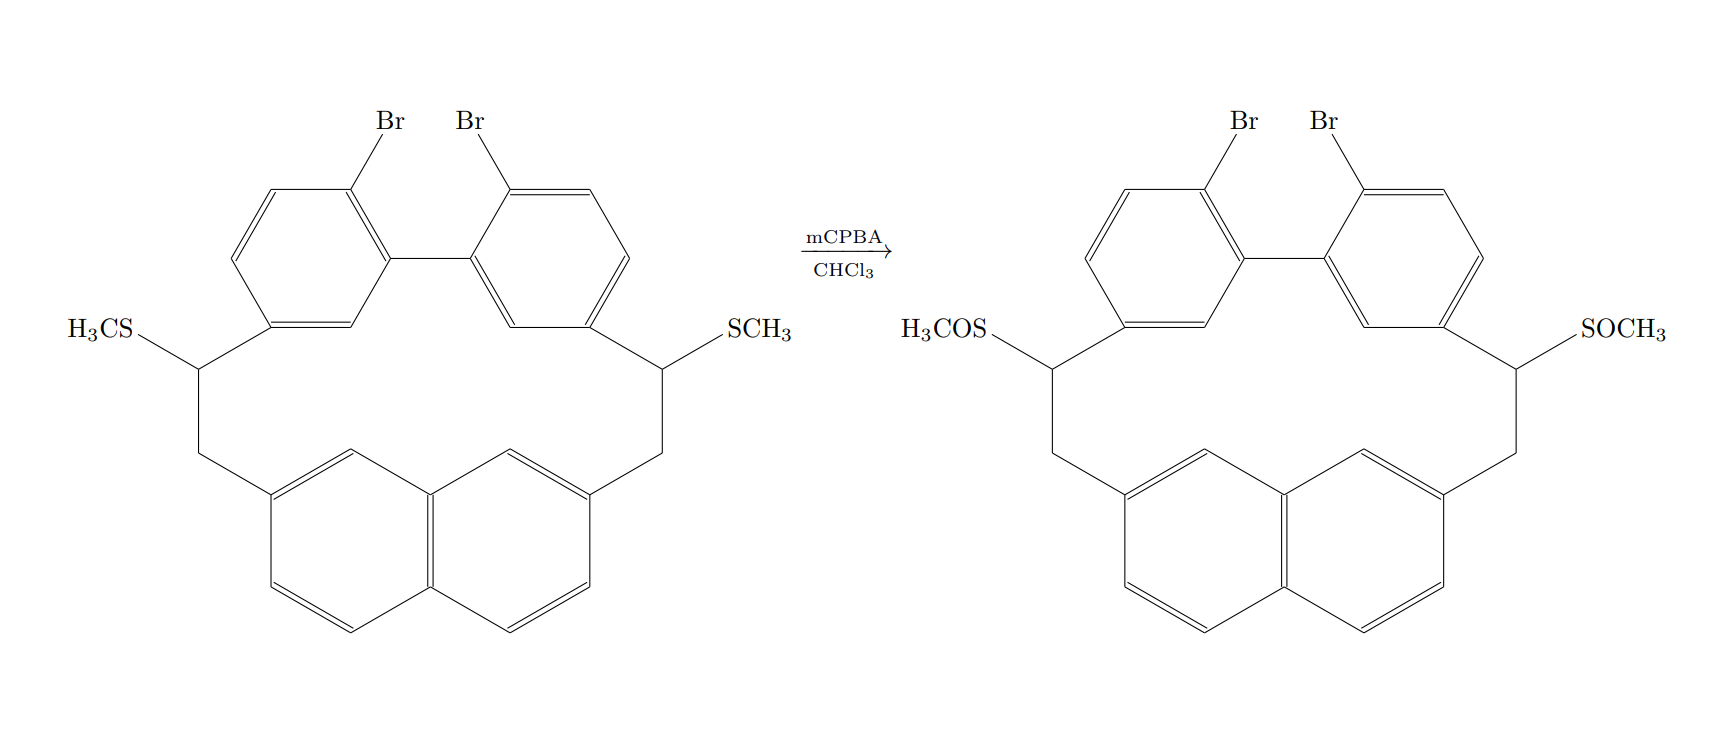
\includegraphics[scale=.45]{thioether_oxidation_overall.PNG}
\end{center}
\end{frame}

\begin{frame}{Thioether Oxidation: Mechanism \#1}
\begin{center}
    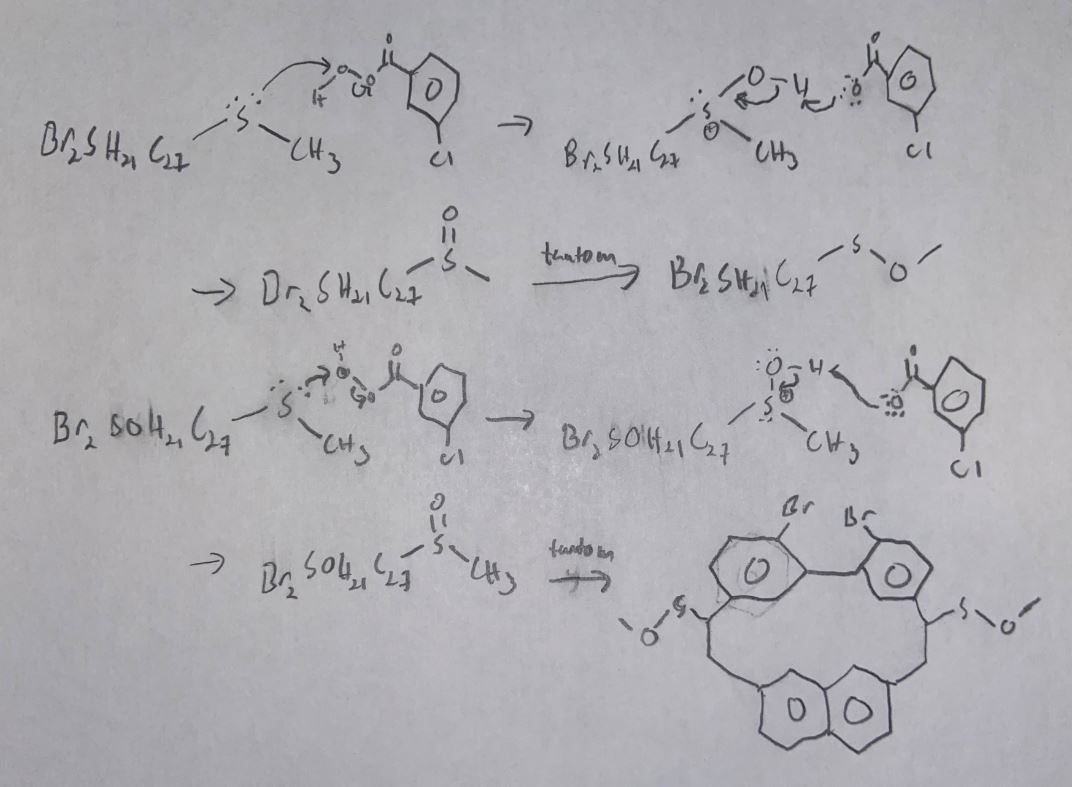
\includegraphics[scale=.35]{Thioether_oxidation_one.JPG}
\end{center}
\end{frame}

\begin{frame}{Sulfenic Ester Elimination}
\begin{center}
    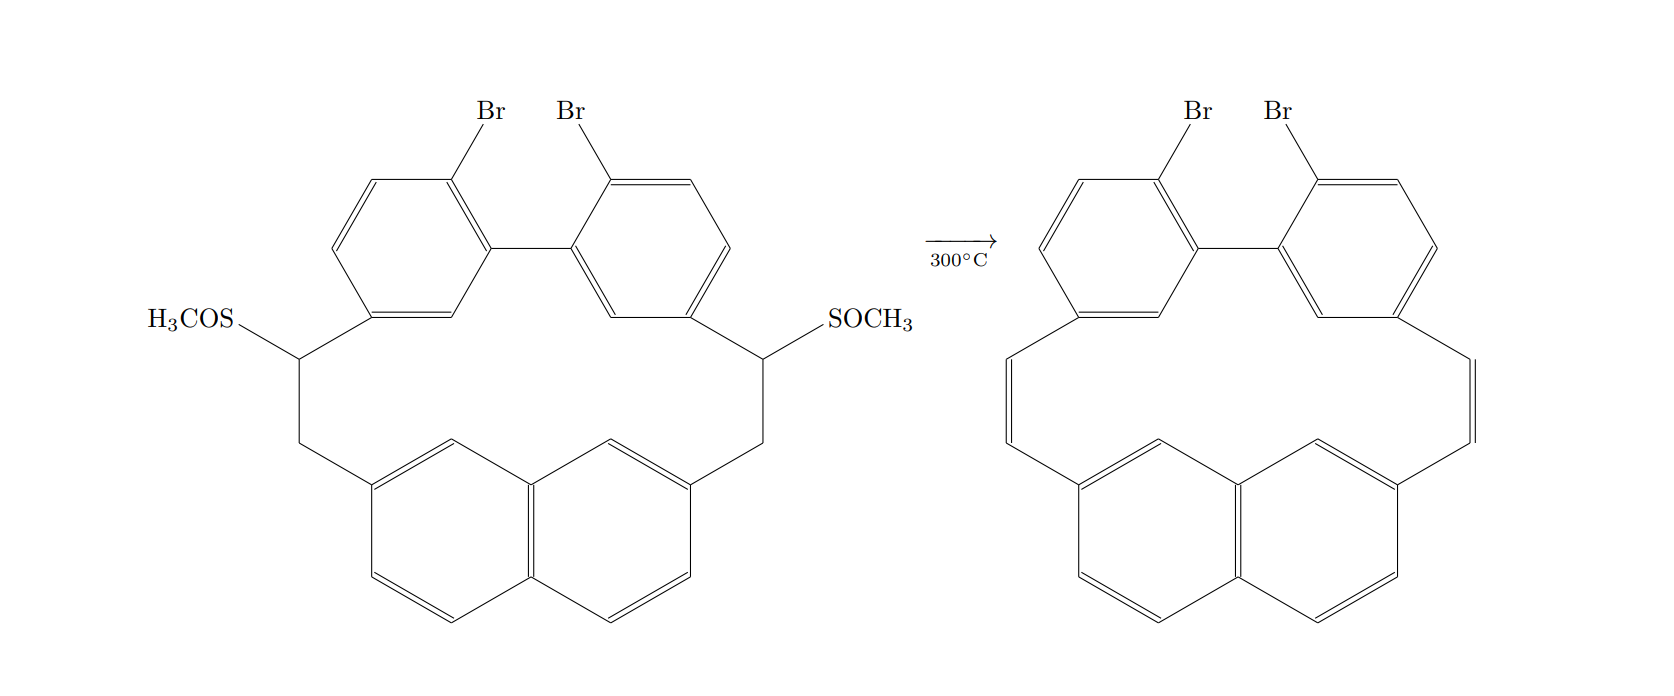
\includegraphics[scale=.46]{sulfenic_ester_elimination_overall.PNG}
\end{center}
\end{frame}

\begin{frame}{Sulfenic Ester Elimination: Mechanism \#1}
\begin{center}
    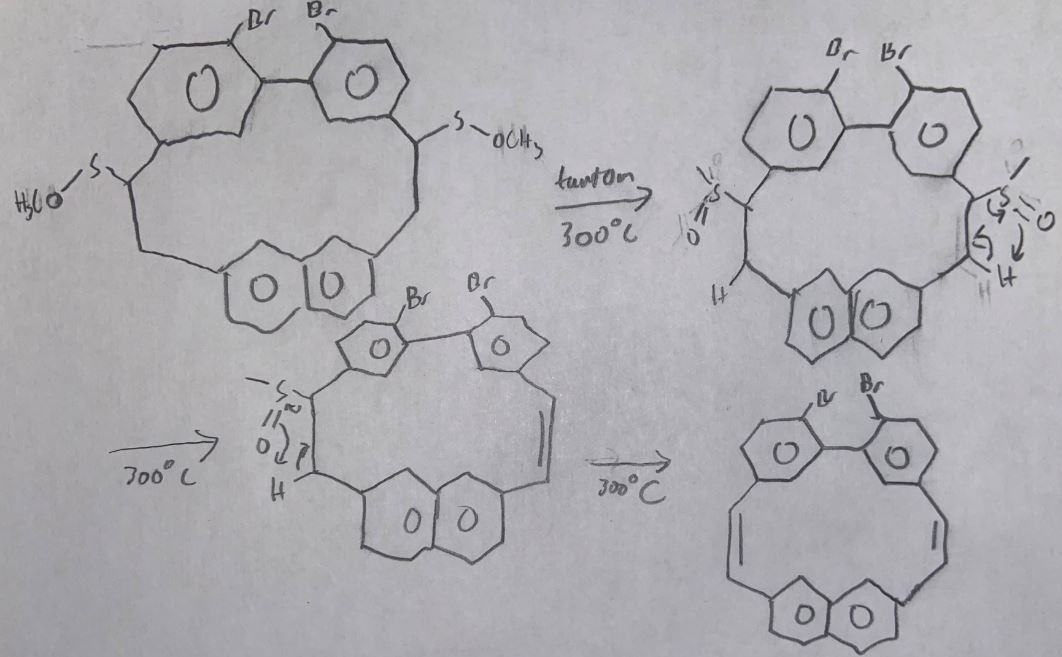
\includegraphics[scale=.37]{sulfinic_ester_elimination one.JPG}
\end{center}
\end{frame}

\begin{frame}{Polyaromatic Cyclization}
\begin{center}
    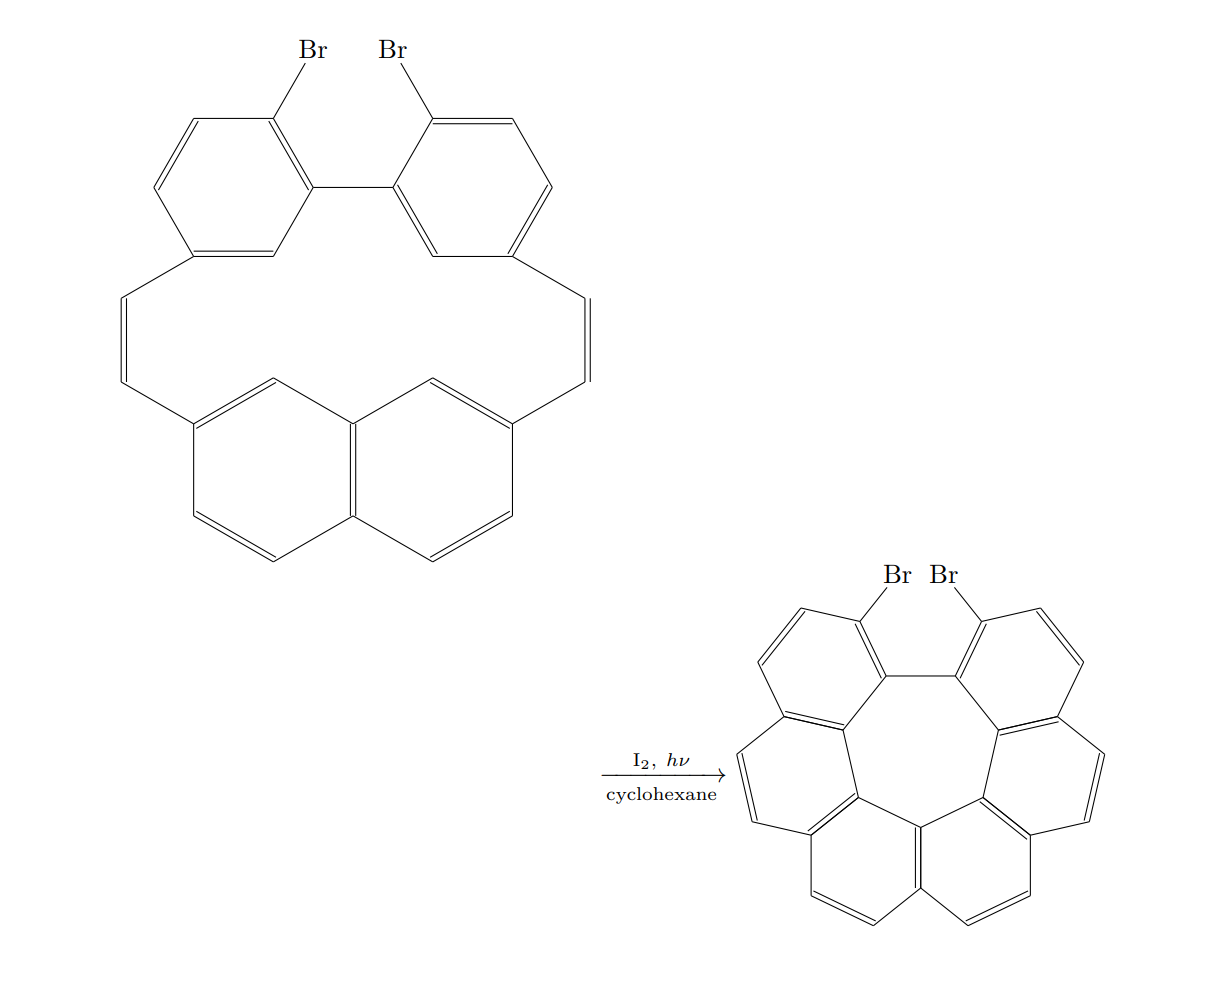
\includegraphics[scale=.43]{polyaromatic_cyclization_overall.PNG}
\end{center}
\end{frame}

\begin{frame}{Polyaromatic Cyclization: Mechanism \#1}
\begin{center}
    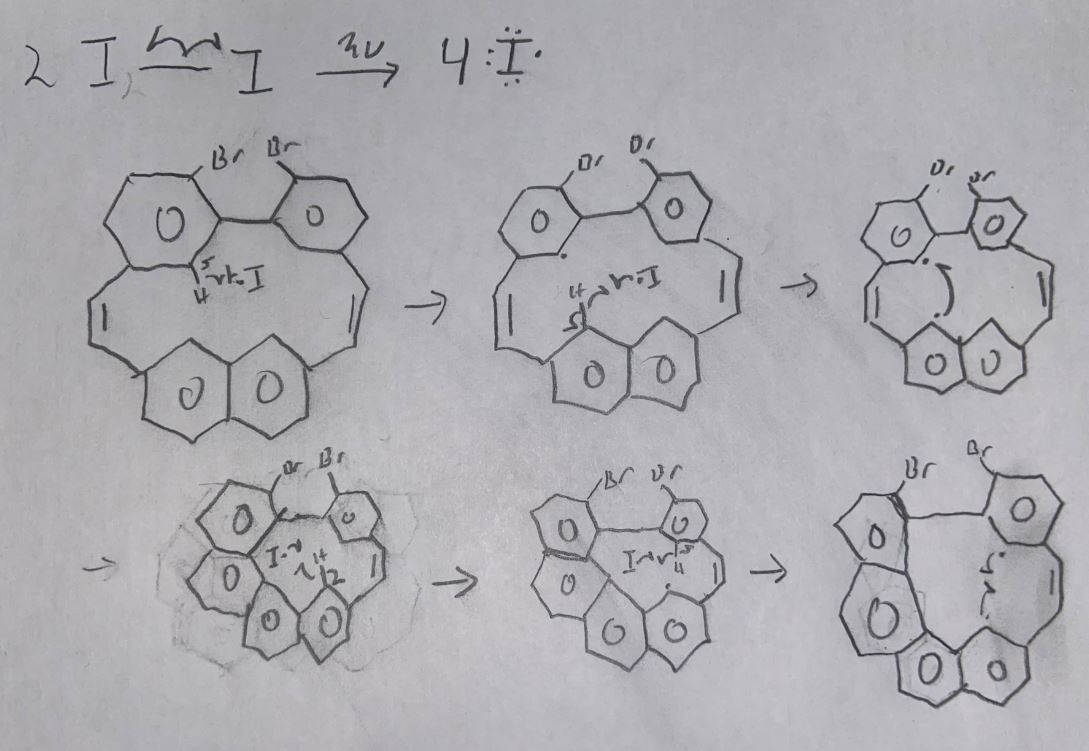
\includegraphics[scale=.36]{polyaromatic_cyclization_one.JPG}
\end{center}
\end{frame}

\begin{frame}{Polyaromatic Cyclization: Mechanism \#2}
\begin{center}
    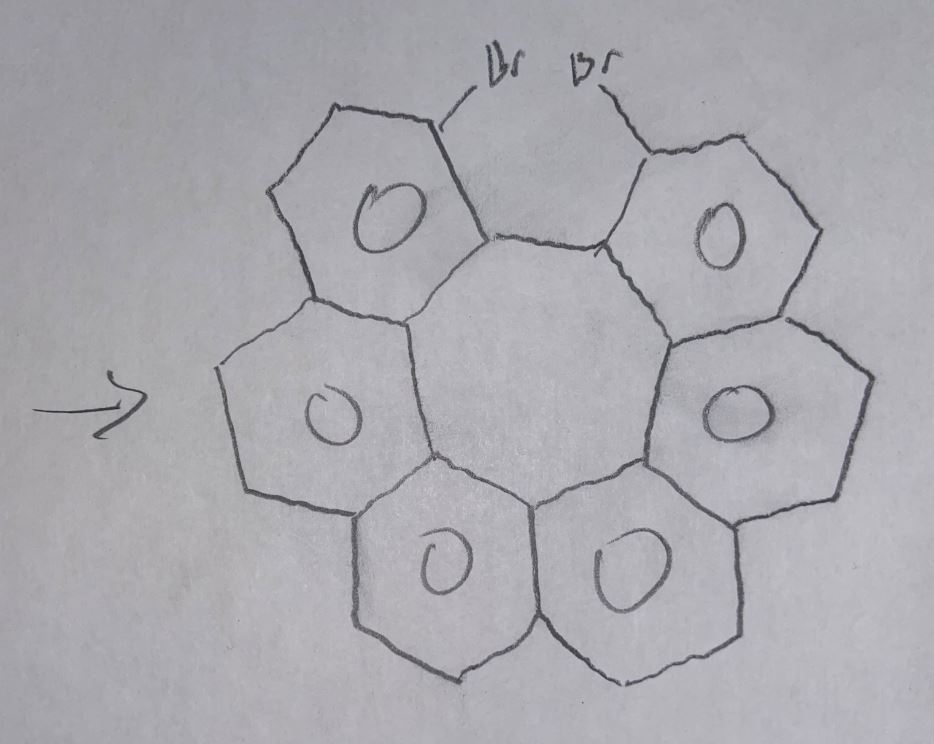
\includegraphics[scale=.43]{polyaromatic_cyclization_two.JPG}
\end{center}
\end{frame}


\begin{frame}{Bouveault Aldehyde Synthesis}
\begin{center}
    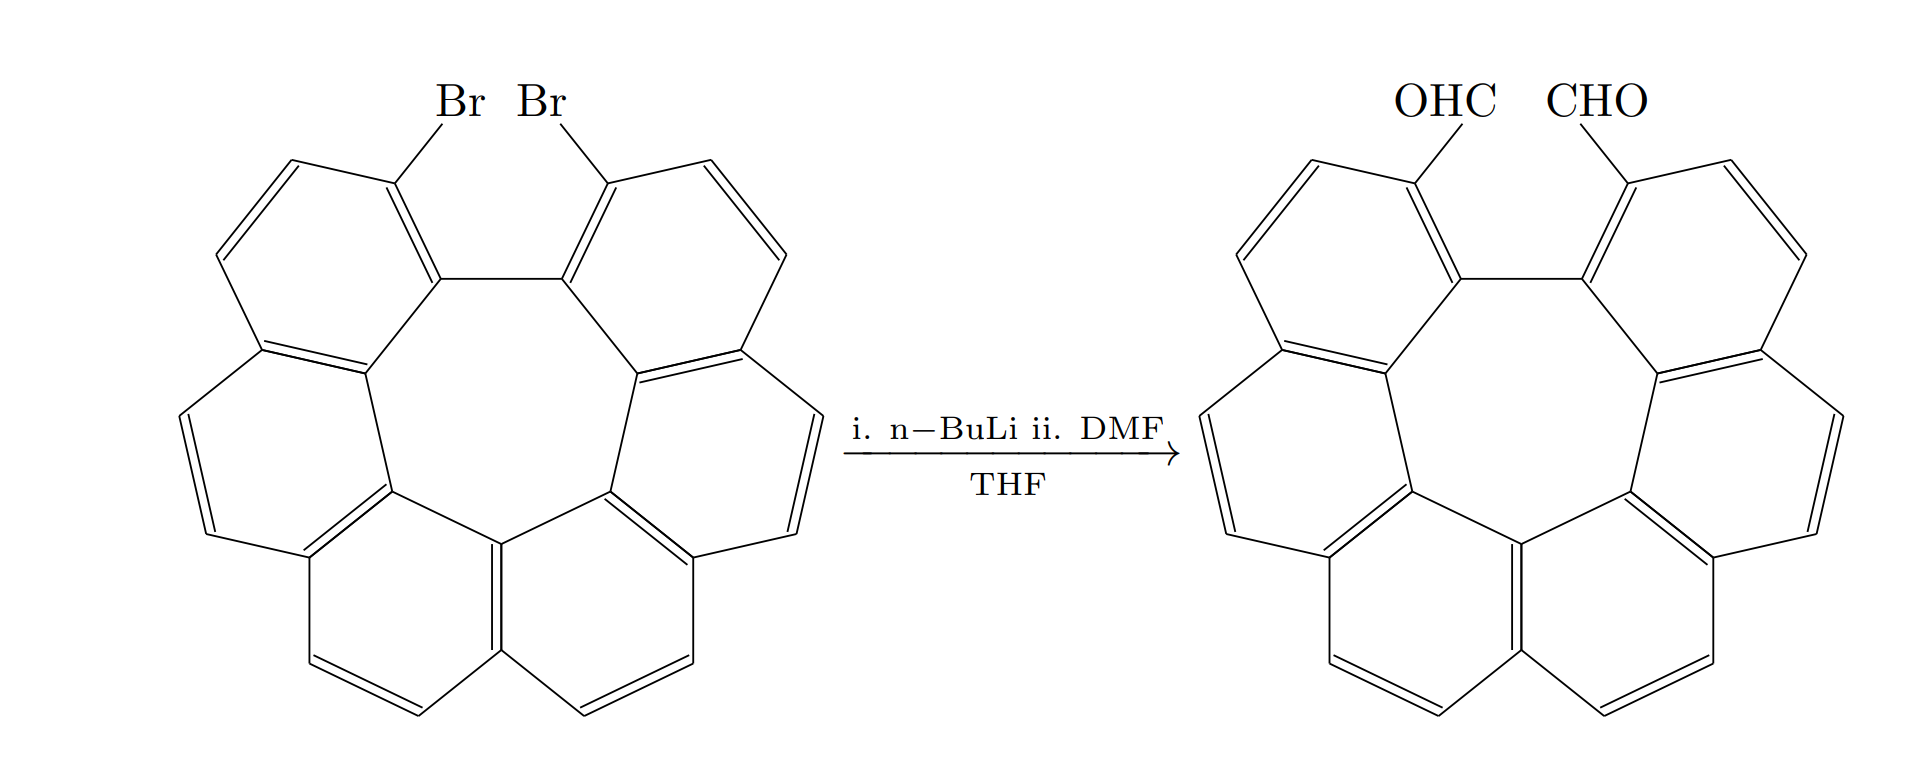
\includegraphics[scale=.45]{bouveault_aldehyde_synthesis_overall.PNG}
\end{center}
\end{frame}

\begin{frame}{Bouveault Aldehyde Synthesis: Mechanism \#1}
\begin{center}
    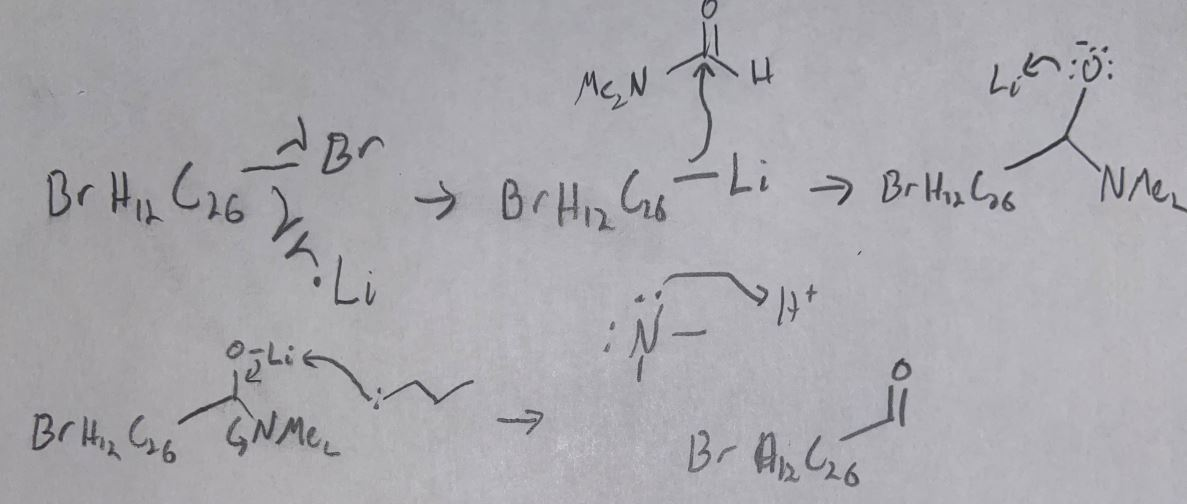
\includegraphics[scale=.37]{bouveault_aldehyde_sythesis_one.JPG}
\end{center}
\end{frame}

\begin{frame}{Bouveault Aldehyde Synthesis: Mechanism \#2}
\begin{center}
    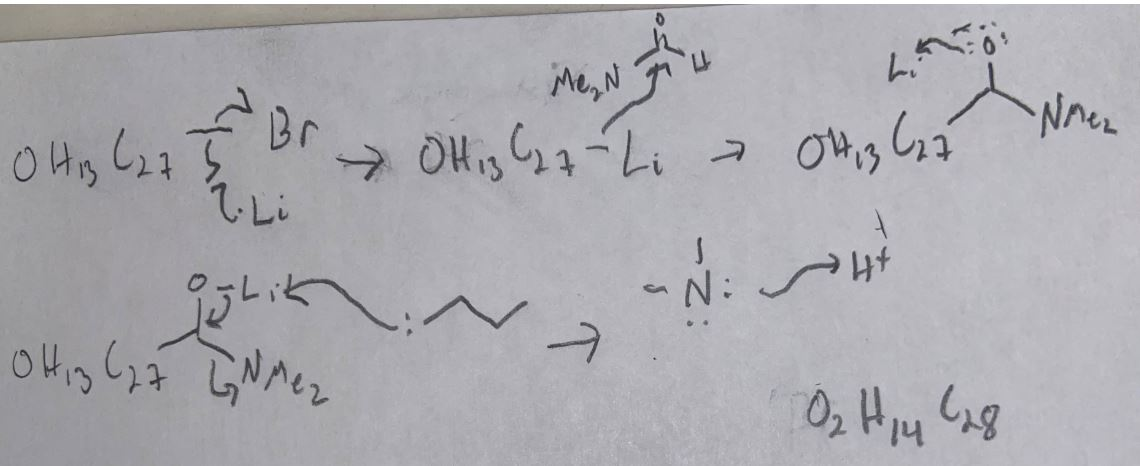
\includegraphics[scale=.37]{bouveault_aldehyde_sythesis_tow.JPG}
\end{center}
\end{frame}

\begin{frame}{McMurry Reaction}
\begin{center}
    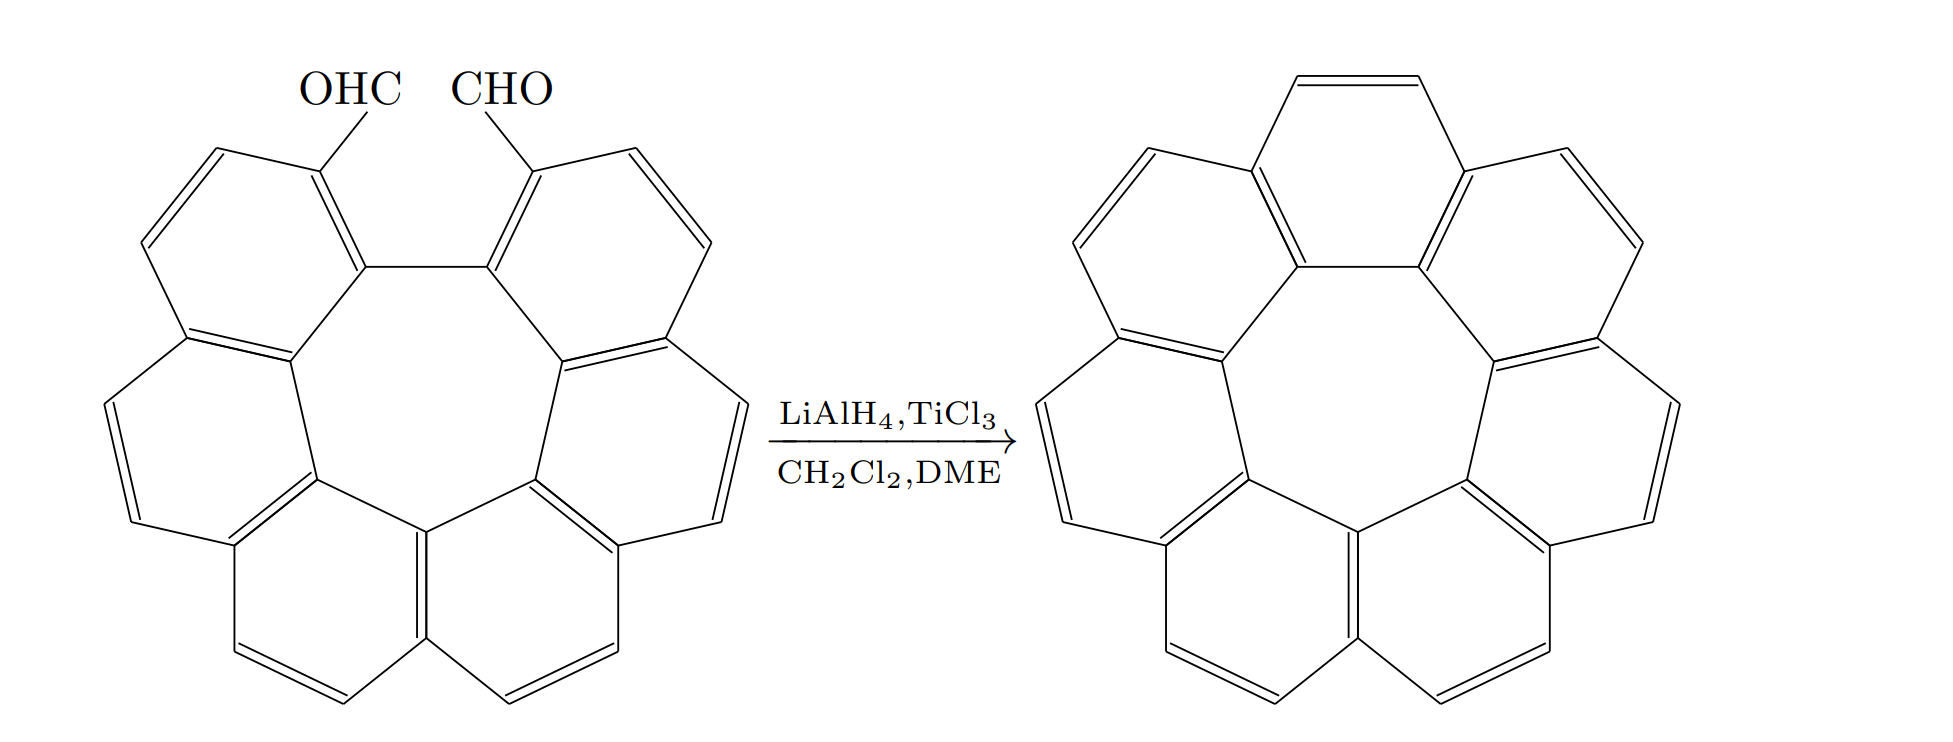
\includegraphics[scale=.45]{mcmurry_reaction_overall.PNG}
\end{center}
\end{frame}

\begin{frame}{McMurry Reaction: Mechanism \#1}
\begin{center}
    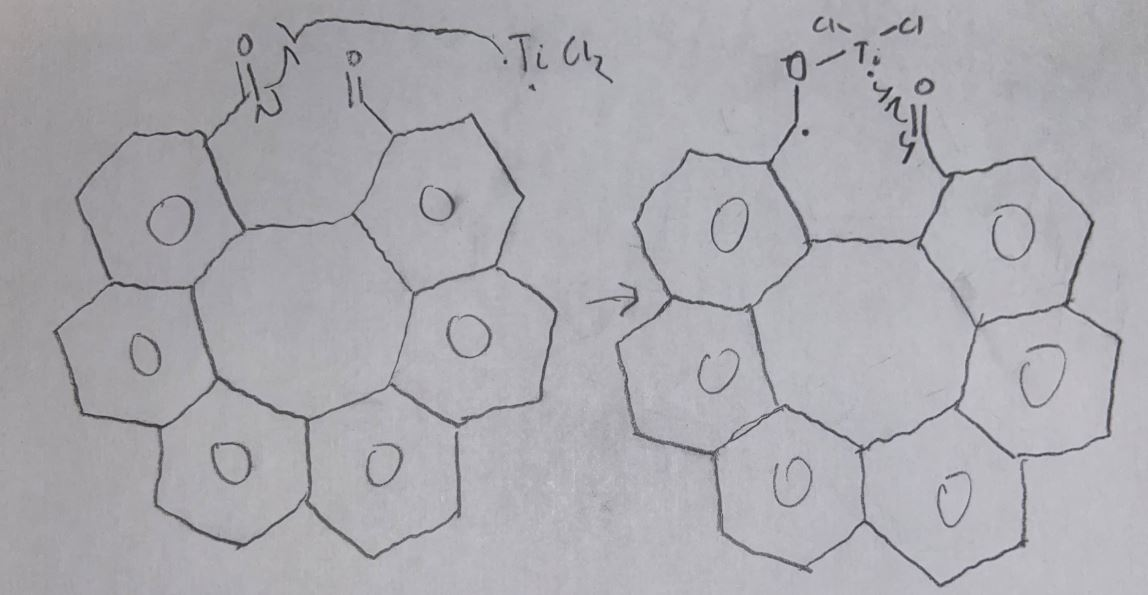
\includegraphics[scale=.35]{mcmurry_reaction_one.JPG}
\end{center}
\end{frame}

\begin{frame}{McMurry Reaction: Mechanism \#2}
\begin{center}
    \includegraphics[scale=.35]{mcmurry_reaction_two.JPG}
\end{center}
\end{frame}

\begin{frame}{McMurry Reaction: Mechanism \#3}
\begin{center}
    \includegraphics[scale=.35]{mcmurry_reaction_three.JPG}
\end{center}
\end{frame}



\begin{frame}{References}
\begin{itemize}
\item
Koji, Yamamoto; Tadashi, Harada; Yoshio, Okamoto; Hiroaki, Chikamatsu; Masao, Nakazaki; Yasushi, Kai; Takuo, Nakao; Mitsuya, Tanaka; Shigeharu, Harada; Nobutami, Kasai (1988). "Synthesis and molecular structure of [7]circulene". \textit{Journal of the American Chemical Society}. 110 (11): 3578–3584. doi:10.1021/ja00219a036

\item
 F. Ullmann; Jean Bielecki (1901). "Ueber Synthesen in der Biphenylreihe".\textit{Chemische Berichte}. 34 (2): 2174–2185. doi:10.1002/cber.190103402141
 
\item
 Smith, Michael B.; March, Jerry (2007), \textit{Advanced Organic Chemistry: Reactions, Mechanisms, and Structure} (6th ed.), New York: Wiley-Interscience, ISBN 978-0-471-72091-1
 \item
 "Global Graphene Market Size is Expected to Reach 151.4 Million and Register a CAGR of 47.7 percent by 2021, Market Trends, Growth and Forecast - Valuates Report". PR Newswire. Cision. 25 November 2019. Retrieved 29 January 2020.
\end{itemize}
    
\end{frame}

\begin{frame}{References}
\begin{itemize}
    \item 
    \textit{Synarchive.} Beaudoin, Daniel. "Synthesis of [7]Circulene". 2011.
    \item
    Karadakov, Peter B. (February 2016). "Do large polycyclic aromatic hydrocarbons and graphene bend? How popular theoretical methods complicate finding the answer to this question" (PDF). \textit{Chemical Physics Letters.} 646: 190–196. doi:10.1016/j.cplett.2015.12.068.
    \item
    David R. Lide (ed), \textit{CRC Handbook of Chemistry and Physics}, 84th Edition. CRC Press. Boca Raton, Florida, 2003; Section 10, Atomic, Molecular, and Optical Physics; Ionization Potentials of Atoms and Atomic Ions
    \item
    http://www.chemgapedia.de/vsengine/vlu/vsc/en/ch/2/vlu/oxidation_reduktion/sulf_oxi.vlu/Page/vsc/en/ch/2/oc/reaktionen/formale_systematik/oxidation_reduktion/oxidation/addition_sauerstoff/oxidation_sulfid_sulfoxid_sulfon/mechanismus.vscml.htm

\end{itemize}
\end{frame}

\begin{frame}{References}
\begin{itemize}
    \item https://chem.libretexts.org/Bookshelves/Organic_Chemistry/Map3A_Organic_Chemistry_(Wade)/133A_Structure_and_Synthesis_of_Alcohols/13.103A_Thiols_(Mercaptans)
    \item 
    March's Organic Chemistry
    \item
    \textit{Name Reactions}: A Collection of Detailed Reaction Mechanisms
By Jie Jack Li
    \item
    https://sci-hub.tw/https://pubs.acs.org/doi/10.1021/jo0160625
    
\end{itemize}
    
\end{frame}


 


\end{document}
